\def\draft{1}

\ifnum\draft=0

% \newcommand{\compacttitlespacing}{0} %disable when we need room for authors
\documentclass[sigconf,anonymous]{acmart}
\settopmatter{printacmref=false}

\else

\documentclass[a4paper]{article}
\usepackage[margin=1in]{geometry}

\fi

\usepackage[english]{babel}
\usepackage[T1]{fontenc}
\usepackage{booktabs}
\usepackage{float}
\usepackage{xcolor}
\usepackage{graphicx}
\DeclareGraphicsExtensions{%
    .png,.PNG,%
    .pdf,.PDF,%
    .jpg,.mps,.jpeg,.jbig2,.jb2,.JPG,.JPEG,.JBIG2,.JB2}
\usepackage{textcomp,amssymb,latexsym}
% \usepackage{amsfonts}
\usepackage{fancyhdr}
\usepackage{enumerate}
\usepackage[ruled,vlined]{algorithm2e}
\usepackage{algpseudocode}
\usepackage{xparse} % argument parsing -- \edist
\usepackage{xspace}
\usepackage{multirow}
\usepackage{csvsimple}
\usepackage{balance} 
\usepackage{diagbox}
\usepackage{amsmath,amsthm}
\usepackage{longtable}
\usepackage{graphicx}
\usepackage{mathdots}

%%%% Type set code and data diagrams
\usepackage{bytefield}
\usepackage{minted}
\usepackage{tabularx}
%%%% Tikz variables, pgfplot
\usepackage{
  tikz,
  pgfplots,
  pgfplotstable
}
\usepgfplotslibrary{statistics}
\usetikzlibrary{
  shapes.geometric,
  shapes.misc,
  arrows,
  external,
  pgfplots.groupplots,
  matrix,
  positioning,
  fit,
  calc,
  decorations.text
}
\pgfplotsset{compat=1.9}

\usepackage{hyperref}
\usepackage[capitalize]{cleveref}

\newcommand*{\email}[1]{\href{mailto:#1}{\nolinkurl{#1}} }
\usepackage{authblk}
\usepackage{blindtext}

\providecommand{\keywords}[1]
{
  \small	
  \textbf{\textit{Keywords---}} #1
}

\usepackage{xparse}
\usepackage{bm}

%%%%%%%%%%%%%%%%%%%%%%%%%%%%%%%%%%%%%%%%%%%%%%%%%%%%%%%%%%%%%%%%%%%%%%%%%%%%%%%%
%%%% Fonts and symbols
%%%%%%%%%%%%%%%%%%%%%%%%%%%%%%%%%%%%%%%%%%%%%%%%%%%%%%%%%%%%%%%%%%%%%%%%%%%%%%%%
\newcommand\funcfont{\textsf}
\newcommand\variablefont{\texttt}


%
% New theorem types: (Already in CCS template)
%
\newtheorem{observation}{Observation}
%\newtheorem{definition}{Definition}
\newtheorem{claim}{Claim}
\newtheorem{assumption}{Assumption}
\newtheorem{fact}{Fact}
\newtheorem{remark}{Remark}
\ifnum\draft=0

\else

\newtheorem{definition}{Definition}
\newtheorem{theorem}{Theorem}[section]
\newtheorem{lemma}{Lemma}[section]
\newtheorem{corollary}{Corollary}[section]
\newtheorem{proposition}{Proposition}
\newtheorem{example}{Example}

\fi

\newcommand{\fixme}[1]{{\textcolor{red}{[FIXME: #1]}}}
\newcommand{\todo}[1]{{\textcolor{red}{[TODO: #1]}}}

\newcommand\ignore[1]{\iffalse#1\fi}


\newcommand{\Hfuzzy}{{\mathrm{H}}^{\rm fuzz}}
\newcommand{\Hminfuzzy}{{\mathrm{H}}^{{\rm{fuzz}}}_{t,\infty}}
\newcommand{\Hpfuzzy}{{\mathrm{H}}^{{\rm{pfuzz}}}}
\newcommand{\Hinf}{{\bf H}^{{\rm \min}}_{\infty}}
\newcommand{\Hminpfuzzy}{{\bf H}^{{\rm pfuzz}}_{t,\infty}}
\newcommand{\BW}{{\rm BW}}
\newcommand{\RBW}{{\rm RBW}}

\newcommand{\pk}{\ensuremath{\mathbf{PK}}\xspace}
\newcommand{\sk}{\ensuremath{\mathbf{SK}}\xspace}


\newcommand{\SPHINCSP}{\texorpdfstring{\ensuremath{\text{SPHINCS}^{+}}\xspace}{SPHINCS+}}
\newcommand{\SPHINCSA}{\texorpdfstring{\ensuremath{\text{SPHINCS-}{\alpha}\xspace}}{SPHINCS-Alpha}}
\newcommand{\WOTSP}{\texorpdfstring{\ensuremath{\text{WOTS}^{+}\xspace}}{WOTS+}}
\newcommand{\WOTSCS}{\texorpdfstring{\ensuremath{\text{CS-WOTS}^{+}}\xspace}{CS-WOTS+}}
\newcommand{\XMSS}{\texorpdfstring{\ensuremath{\text{XMSS}}\xspace}{XMSS}}
\newcommand{\XMSSMT}{\texorpdfstring{\ensuremath{\text{XMSS}^\text{MT}}\xspace}{XMSSMT}}
\newcommand{\secpara}{\ensuremath{\lambda}\xspace}
\newcommand{\Th}{\ensuremath{\mathbf{T}}\xspace}
\newcommand{\hashH}{\ensuremath{\mathbf{H}}\xspace}
\newcommand{\hashF}{\ensuremath{\mathbf{F}}\xspace}
\newcommand{\PRF}{\ensuremath{\mathbf{PRF}}\xspace}
\newcommand{\PRFmsg}{\ensuremath{\mathbf{PRF_{msg}}}\xspace}
\newcommand{\hashmsg}{\ensuremath{\mathbf{H_{msg}}}\xspace}
\newcommand{\bool}{\ensuremath{\{0,1\}}\xspace}
\newcommand{\byte}{\ensuremath{\mathbb{B}}\xspace}
\newcommand{\ADRS}{\ensuremath{\mathtt{ADRS}}\xspace}
\newcommand{\md}{\ensuremath{\mathtt{md}}\xspace}
\newcommand{\seed}{\ensuremath{\mathtt{seed}}\xspace}
\newcommand{\len}{\ensuremath{\mathtt{len}}\xspace}
\newcommand{\prf}{\ensuremath{\mathtt{prf}}\xspace}
\renewcommand{\root}{\ensuremath{\mathtt{root}}\xspace}
\newcommand{\sig}{\ensuremath{\mathtt{SIG}}\xspace}
\newcommand{\sight}{\ensuremath{\mathtt{SIG}_\mathtt{HT}}\xspace}
\newcommand{\sigots}{\ensuremath{\mathtt{SIG}_\mathtt{OTS}}\xspace}
\newcommand{\sigxmss}{\ensuremath{\mathtt{SIG}_\mathtt{XMSS}}\xspace}
\newcommand{\sigfors}{\ensuremath{\mathtt{SIG}_\mathtt{FORS}}\xspace}
\newcommand{\randstr}{\ensuremath{\mathtt{R}}\xspace}

\newcommand{\thinf}{{\widetilde{\mathbf{H}}_{\infty}}}
\newcommand{\hinf}{{{\mathbf{H}}_{\infty}}}
\newcommand{\eqdef}{\stackrel{\rm def}{=}}
\newcommand{\kaiyi}[1]{{\color{cyan} Kaiyi } {\color{blue} #1}}
\newcommand{\cui}[1]{{\color{cyan} Cui } {\color{blue} #1}}

%%%%%%%%%%%%%%%%%%%%%%%%%%%%%%%%%%%%%%%%%%%%%%%%%%%%%%%%%%%%%%%%%%%%%%%%%%%%%%

\newtheorem{construction}{Construction}[section]


\newcommand{\authnote}[2]{\textcolor{red}{\textsf{#1 }\textcolor{blue}{ #2}}}
\newcommand{\yu}[1]{{\authnote{Yu}{#1}}}
%\newcommand{\kaiyi}[1]{{\authnote{Kaiyi}{#1}}}

\begin{document}
%\fontfamily{lmr}\selectfont
\fancyhead{}
\def\thetitle{SPHINCS-alpha \\ Submission to the NIST post-quantum project}
\title{\thetitle}
\date{\today}
\author{The SPHINCS-alpha Team}

\maketitle

\newpage

\tableofcontents

\newpage

% Section I
\section{Introduction} \label{sec:intro}

Hash-based signature is one of the most promising candidates for (and perhaps the most conservative approach to)  post-quantum digital signatures. An advantage of hash-based signatures is that its (classical as well as quantum) security strength is better understood (and easier to evaluate) than other candidates, by solely relying on the idealized hardness\footnote{The design philosophy of symmetric primitives (including hash functions) is that they should only admit generic attacks, otherwise the design is considered to be flawed.} of the cryptographic hash functions.  

\paragraph{Stateful signatures.} Ralph Merkle proposed a hash-based signature \cite{C:Merkle89a} that builds upon Lamport's one-time signature (OTS) \cite{Lamport79}. The recent efforts towards improving stateful signatures lead to the eXtended Merkle Signature Scheme (XMSS)~\cite{hulsing2018xmss} and the Leighton-Micali Signature (LMS)~\cite{mcgrew2019leighton},  standardized by NIST~\cite{cooper2020recommendation} and IETF.

\paragraph{Stateless signatures.} In a typical stateful signature, e.g., Merkle's signature scheme (MSS), the signer keeps track of which private key of the OTS has been used to avoid security issues from subsequent reuse. This is however not always possible in many practical scenarios. Goldreich proposed a stateless hash-based signature construction~\cite{C:Goldreich86a,Goldreich04} which removes the need for maintaining a local state but results in prohibitively large signatures. Recently,  this line of research gets renewed interest. By incorporating the hypertree structure, SPHINCS~\cite{EC:BHHLNP15} offered a practical instantiation of the Goldreich-style stateless hash-based signature.  SPHINCS serves as a basis for subsequent works driven by the NIST PQC standardization process, including Gravity-SPHINCS~\cite{RSA:AumEnd18}, SPHINCS-Simpira~\cite{EPRINT:GueMou17} and \SPHINCSP\ \cite{CCS:BHKNRS19}. Among these schemes, \SPHINCSP employs a new design framework based on few-time signature (FTS), and a new security analysis framework from ``tweakable hash function''. It is generally considered as the current state-of-the-art of stateless hash-based signatures and is to be standardized by NIST.

\ignore{
\paragraph{Performance.} Despite the desirable features such as conservative assumptions, well-understood security, and flexibility in choosing the underlying hash functions,  the performance of hash-based signatures, in terms of signing
speed and signature size, is less competitive than 
other (e.g., lattice-based) candidates, which makes it less favorable for adoption. The performance of a hash-based signature can benefit from 
new structures~\cite{AC:BleMau96,bleichenbacher1996optimal,PQCRYPTO:BucDahHul11}, more
efficient underlying components (e.g., one-time signature~\cite{IMA:DodSmaSta05,AFRICACRYPT:Hulsing13},  few-time signature~\cite{CCS:Perrig01,ACISP:ReyRey02}, lightweight hash function~\cite{ToSC:KLMR16}), and hardware accelerations~\cite{PKC:HulRijSch16,PQCRYPTO:Kolbl18,SAC:WJWDGSN19,TCHES:AmiCurZbi18,TCHES:BHRV21,sun2020efficient}.  The main focus of this paper is algorithmic optimization of stateless hash-based signatures. 
}

\ifnum\draft=0

\begin{table*}[ht]
    \centering
    \caption{Performance comparison between \SPHINCSP\ and \SPHINCSA, with simple tweakable hash function instantiated with \textsf{sha256}. Key generation, signing and verification time are in terms of CPU cycles; public key, secret key and signature size are in bytes. All cycle counts are the median of 100 runs.}
    \label{tab:comp tiny}
    \begin{tabular}{c rrrr rrrr rrrr}%
    \toprule
       & \multicolumn{4}{c}{\SPHINCSP}  & \multicolumn{4}{c}{\SPHINCSA}  &\multicolumn{4}{c}{Relative Change} \\ %\cmidrule{2-5} \cmidrule{6-9} \cmidrule{10-13} 
      Param. &  KeyGen & Sign & Verify & Size &  KeyGen & Sign & Verify & Size &  KeyGen & Sign & Verify & Size\\ \midrule
      \csvreader[head to column names]{data/compare-mini.csv}{}% use head of csv as column names
      { \nameone  & $\keygenone$ & $\signone$ &$\verifyone$ & \signatureone & $\keygentwo$ & $\signtwo$ &$\verifytwo$ & \signaturetwo & \keygenratio & \signratio &\verifyratio & \signatureratio \\}%
     \vspace{-1em} \\ \bottomrule
    \end{tabular}
\end{table*}

\else
\begin{table}[th]
    \centering
    \caption{Performance comparison between \SPHINCSP\ and \SPHINCSA, with simple tweakable hash function instantiated with \textsf{shake}. Key generation, signing and verification time are in terms of CPU cycles; public key, secret key and signature size are in bytes. All cycle counts are the median of 100 runs.}
    \label{tab:comp tiny}
    \resizebox{\columnwidth}{!}{%
    \begin{tabular}{c rrrr rrrr rrrr}%
    \toprule
       & \multicolumn{4}{c}{\SPHINCSP}  & \multicolumn{4}{c}{\SPHINCSA}  &\multicolumn{4}{c}{Relative Change} \\ %\cmidrule{2-5} \cmidrule{6-9} \cmidrule{10-13} 
      Param. &  KeyGen & Sign & Verify & Size &  KeyGen & Sign & Verify & Size &  KeyGen & Sign & Verify & Size\\ \midrule
      \csvreader[head to column names]{data/compare-mini.csv}{}% use head of csv as column names
      { \nameone  & $\keygenone$ & $\signone$ &$\verifyone$ & \signatureone & $\keygentwo$ & $\signtwo$ &$\verifytwo$ & \signaturetwo & \keygenratio & \signratio &\verifyratio & \signatureratio \\}%
     \vspace{-1em} \\ \bottomrule
    \end{tabular}%
    }
\end{table}

\fi


%\subsection{Our Contributions}
\paragraph{Summary of our Work.}
We propose \SPHINCSA, a stateless hash-based signature scheme, which improves upon the state-of-the-art stateless hash-based signature scheme \SPHINCSP, while preserving the core elements that made the original \SPHINCSP a standout project. 

Our optimization mainly stems from the optimization of the one-time signature scheme, which we prove to have a size-optimal encoding scheme among all tree structured one-time signatures. Moreover, no DAG-based construction offers better size efficiency, making our proposal size-optimal among all known schemes to the best of our knowledge \cite{optimalwots}.

Since our modification upon the \SPHINCSP scheme is limited to the encoding scheme of the underlying \WOTSP one-time signature, the security analysis of our new scheme remains largely the same as the original analysis.
Based on the security analysis of the original work, we estimate the security level and carefully choose parameters in order to achieve optimized performance.

To facilitate a fair comparison, we implement \SPHINCSA\ by adapting the code of \SPHINCSP\ and compare their performance on a desktop computer. As shown in \cref{tab:comp tiny}, under the ``small'' series parameters (optimized towards small signature size) our scheme reduces signature size and running time by 8-12\% and 2-16\% respectively at all security levels while under the ``fast'' series (optimized towards fast signing operations) our scheme exhibits better performance in general. 

We refer to more detailed comparisons for the full spectrum of parameter choices in \cref{sec:performance}.
As summarized in \cref{tab:bench comp}, our scheme offers an overall performance improvement for most parameter settings, in terms of signing time and signature size. On the downside, we experience an up to 253\% increase in verification time. Nevertheless, we argue that for specific scenarios where verification time is critical, we can re-tune the parameters towards fast verification. 
%since the verification only amounts to 1-9\% of the signing time we argue that this sacrifice is worthwhile considering efficiency gain in signing time and signature size.

\paragraph{Other Changes Made.}
Following the decisions made by NIST~\cite{nistdecision}, we remove haraka and robust version from tweakable hash function.

\paragraph{Acknowledgement.}

We acknowledge the \SPHINCSP team for their great work on the original \SPHINCSP project.  A significant portion of our code and documentation derives from their commendable efforts.    % basic introduction
%\section{Preliminary}
\input{revisit}
\section{\SPHINCSA\ vs. \SPHINCSP} \label{sec:balanced wotsp}

In this section we highlight our improvement upon the original \SPHINCSP\ scheme, namely, the one-time signature component.
Our optimized scheme, \WOTSCS, allows a larger message space / signature size ratio as compared to the original \WOTSP\ scheme, allowing a smaller one-time signature size. As a result, the parameters of the hash-based signature scheme can thus be re-tuned to reduce the signature size without exacerbating the computation time.

We explain the details of our optimization as well as some technical proofs in this section.

\subsection{The \WOTSP~Encoding}

The reason that the \WOTSP (as well as other Winternitz-type OTS) scheme introduces the checksum is that in absence of the checksum the adversary can efficiently forge signatures given a single pair of valid message signature. That is, given $(\sigma,m)$ he forges any $m'$ satisfying $\forall i(m_i\leq m'_i)$ by computing $\hashF^{m'_i}(sk_i)$ $=\hashF^{m'_i-m_i}\big( \hashF^{m_i}(sk_i)\big)$.

\ignore{
The adversary has advantages in the \WOTSP (as well as other Winternitz type one time signature scheme) if there is no checksum. It can easily obtain $\hashF^{m'_i}(sk_i)$ forall $m'_i$ such that $ m_i\leq m'_i$ from a valid pair of signature and message $(\sigma,m)$. That means the adversary can forge any $m'$ such that $\forall i,m_i\leq m'_i$.
}
The checksum addresses the issue: an increase in any $m_i$ leads to a decrease in at least one $C_i$ (recall $C=\sum_{i=1}^{l_1}(w-1-m_i)$). Therefore, the adversary cannot forge any $(m',C')$ satisfying both $\forall i(m_i\leq m'_i)$ and $\forall i(C_i\leq C'_i)$ at the same time.






\subsection{Size-Optimal Encoding}

More formally, the problem of constructing one-time signature reduces to that of building an efficient encoding scheme $\mathsf{Enc}:\mathcal{M}\rightarrow \mathcal{C}\subseteq[w]^{l}$ for some incomparable codeword set $\mathcal{C}$ (see \cref{incomparable}). In case of \WOTSP, the encoding function $\mathsf{Enc}$ simply appends the checksum to the original message. Note that \WOTSP~ fixes the size of the message to $l_1$ (i.e., $\mathcal{M}=[w]^{l_l}$) and then constructs as small codewords as possible (minimizing $l-l_1$). 





\begin{definition}[(In)comparability]\label{incomparable} For  $a,b\in[w]^l$, we denote by $a \leq b$ if for every $ i \in [l]$ we have $a_{i+1}\leq b_{i+1}$.  If $a\leq b$ or $b\leq a$ we say that $a$ and $b$ comparable, or otherwise $a$ and $b$ are incomparable.
A set $S\subseteq\{a:a\in[w]^l\}$ is said to be incomparable (or called an ``antichain'' in order theory terminology) if any two elements of $S$ are incomparable. 
\end{definition}

We take a slightly different approach to encoding the messages. That is, we first fix the size of the codewords to $l$, $\mathcal{C}\subseteq[w]^{l}$, and strive to accommodate as large message space $\mathcal{M}$ as possible. Given that {\sf Enc} is an injection it is essentially to maximize the size of $\mathcal{C}\subseteq[w]^{l}$. A natural approach is to encode the codewords such that 
all elements of every codeword sum to the same value, and therefore the checksum is not explicitly needed.
Bos and Chaum~\cite{C:BosCha92} studied this approach for the special case of $w=2$.  Vaudenay~\cite{vaudenay1993one} generalized it to arbitrary $w$, but he did not provide an encoding algorithm. Perin et al.\ provided a similar encoding algorithm in~\cite{perin2021improved}, but they did not present a size-optimal proof.
%As stated in Theorem~\ref{Eisantichain}, this gives rise to the desired set of codewords.
%following the works of Kaji et al.~\cite{kaji2018hash},
 
 
\begin{theorem}
    \label{Eisantichain}
    For any $m\in[l(w-1)+1]$, 
   $\mathcal{C}_m\eqdef\{v\in [w]^l : \sum_{i=1}^l v_i = m \}$ is incomparable.
\end{theorem}
\begin{proof}
Suppose towards contradiction that $\mathcal{C}_m$ (for some fixed $m\in[l(w-1)+1]$) is not incomparable, then there exist distinct $a,b\in \mathcal{C}_m$ s.t. $a\leq b$. There must be an index $j$ such that $a_j<b_j$ (otherwise $a= b$). However, due to equal sum  $\sum_i a_i=\sum_i b_i$  we have $\sum_{1\leq i\leq l \wedge i\neq j} (a_i-b_i)>0$, and there must exist some $1\leq k\leq l$ such that $a_k>b_k$, which is a contradiction to $a\leq b$. \qed
\end{proof}

Every $\mathcal{C}_m$ gives an encoding scheme but with different size. For $m=0$ or $m=l(w-1)$, $\mathcal{C}_m$
consists of only a single codeword. We argue that the size of $\mathcal{C}_m$ reaches its maximal in the middle, i.e., when $m=\lfloor\frac{l(w-1)}{2}\rfloor$. One easily  verifies that this holds in the binary case (i.e., $w=2$) where $|\mathcal{C}_m|=\binom{l}{m}$. Perin et al.~\cite{perin2021improved} proved that $|\mathcal{C}_{m}|$ reaches its maximum 
when $m=\lfloor\frac{l(w-1)}{2}\rfloor$. We prove a stronger optimality result in Theorem~\ref{sec:con} that the size of $\mathcal{C}_{m}$, when $m=\lfloor\frac{l(w-1)}{2}\rfloor$, is not only the largest in all $\mathcal{C}_m$ for $m\in[l(w-1)+1]$ but the largest among all valid sets of codewords.

\begin{theorem}[Size-optimal encoding]\label{sec:con}
For every incomparable $\mathcal{C^*}\in P([w]^l)$, it holds that 
\[
 |\mathcal{C^*}| \leq |\mathcal{C}_{\lfloor\frac{l(w-1)}{2}\rfloor}|\enspace.
\]
\end{theorem}
We defer its proof to Theorem~\ref{maximum-antichain}, which rephrases
Theorem~\ref{sec:con}  in the language of order theory. Prior to that, we discuss how to compute  $|\mathcal{C}_m|$ by recursion, and give an explicit construction of 
encoding messages into $\mathcal{C}_{m}$ for $m=\lfloor\frac{l(w-1)}{2}\rfloor$. Hereafter, we denote such $\mathcal{C}_{m}$ with maximal size by $\mathcal{C}$ for brevity. 


\ignore{
\begin{construction}[Maximum codeset]\label{sec:con} We let
$$\mathcal{C}\eqdef\{v\in [w]^l : \sum_{i=1}^l v_i = \left\lfloor \frac{l(w-1)}{2} \right\rfloor \} \enspace.$$
\end{construction}
\subsubsection{Construction.}
\label{sec:con}
Our construction for $E$ is

$$E=\{v\in [w]^l : \sum_i v_i = \left\lfloor \frac{l(w-1)}{2} \right\rfloor \}$$
}

%\begin{theorem}
%    \label{Eisantichain}
%    $E$ defined as per Construction~\ref{sec:con} is incomparable.
%\end{theorem}



\paragraph{Counting the size.} Now we need to figure out the size of $\mathcal{C}$. As a special case, $|\mathcal{C}|=\binom{l}{\lfloor l/2 \rfloor}$ when $w=2$. Fix $w$, let
$$ D_{n,m}= |\{v\in [w]^n : \sum_{i=1}^{n} v_i = m \}| \enspace , $$

we have their initial values
\begin{align*}
D_{1,m} &= 1 , \mbox{ for }m\in \{0,1,\dots,w-1\} \\
D_{n,m} &= 0 , \mbox{ for }2\leq n \in \mathbb{Z}, m \in \mathbb{Z^-} \enspace ,
\end{align*}
and recurrence relation
\begin{equation} \label{equ:recurrence}
    D_{n,m} = \sum_{i=0}^{w-1} D_{n-1,m-i} , 2 \leq n \in \mathbb{Z},m\in \{0,1,\dots,l(w-1)\} \enspace . 
\end{equation}

Note when $w=2$, this method is equivalent to recurrence relation of binomial coefficient, i.e., $\binom{n}{m}=\binom{n-1}{m-1}+\binom{n-1}{m}$.

Let us explain the recurrence relation. To compute $D_{n,m}$,  consider the value of its last summand, which could be any value in $\{0,1,\dots,w-1\}$. If this value is set to $i$, the sum of the first $n-1$ elements must be $m-i$. Therefore, we notice that  the problem ``$n$ elements with sum to $m$'' into those ``$n-1$ elements with sum to $m-i$''. Thus we can simply count $D_{n,m}$ by accumulating $D_{n-1,m-i}$.
Following this method, $D_{l,\lfloor l(w-1)/2 \rfloor}$ gives the size of $\mathcal{C}$.

\paragraph{Related works.} $D_{n,m}$ is also the $m$-th coefficient of $(1+x+x^2+\dots+x^{w-1})^n$. Euler~\cite{euler1801evolutione} has studied $w=3,4,5$, known as trinomial, quadrinomial and quintinomial  coefficients respectively. The generalized form was  studied in the literature, e.g.,~\cite{andre1876memoire,warnaar1997andrews,belbachir2020congruence}. Actually, we can use an inclusion-exclusion argument to express it as a function of binomial coefficients~\cite{28861}
$$ D_{n,m} = \sum_{s=0}^{\lfloor{m/w}\rfloor} (-1)^s \binom{n}{s} \binom{m+n-sw-1}{n-1} \enspace .$$

\paragraph{Encoding algorithm.} Now we make the construction explicit by giving an efficient encoding algorithm, which maps a message $x\in [|\mathcal{C}|]$ into an element in $\mathcal{C}$.
We give the pseudocode of the encoding algorithm in \cref{alg:encode}.
\begin{algorithm}
\SetKwProg{func}{Function}{}{end}
\caption{Encode:$[|\mathcal{C}|]\rightarrow\mathcal{C}$.} \label{alg:encode}
\func{{\rm Encode}(x)}{
    Let $v$ be an array of size $l$\;
    $m\gets\lfloor l(w-1)/2 \rfloor$\;
    \For{$i\gets l$~\dots~$1$}{
        \For{$j\gets 0$~\dots~$\min(w-1,m)$}{
            \If{$x\geq D_{i-1,s-j}$}{
                $x\gets x-D_{i-1,s-j}$\;
            }\Else{
                $v_{l-i}\gets j$\;
                {\bf break}\;
            }
        }
        $m\gets m-v_{l-i}$\;
    }
    \Return $v$\;
}
\end{algorithm}

Let us explain the encoding algorithm. As previously stated, the problem can be divided into several subproblems by considering the value of the first element $v_{l-i}$. To encode a natural number $x\in [0,D_{i,m})$, we can simply determine $v_{l-i}=j$ by seeking which $j$ satisfies $x\in [\sum_{k<j}D_{i-1,m-k},\sum_{k\leq j}D_{i-1,m-k})$. Once the value of $v_{l-i}$ is determined, we proceed to the next terms until all elements are decided.

In order to prove the optimality of the encoding,  we need some prerequisites about the order theory. The relationship between one-time signature and order theory has been investigated in \cite{C:BleMau94}.

\paragraph{Preliminaries of Order Theory} 

\begin{definition}[Poset]
A poset ($\mathcal{S}$,$\leq$) consists of a set $\mathcal{S}$ together with an antisymmetric, transitive and reflexive binary relation `$\leq$', where are certain pairs $(x,y)\in\mathcal{S}$ are comparable ($x\leq y$ or $y\leq x$).
\end{definition}
Note that a poset does not require all pairs in $\mathcal{S}$ to be comparable, and thus it is also known as a partially ordered set. 

\begin{definition}[(Anti)chain and decomposition]
A chain (resp., antichain) refers to a subset of a poset, whose every pair of elements is comparable (resp., incomparable). A chain decomposition is a partition of a poset into disjoint chains.
\end{definition}

\ignore{
A partially ordered set (poset) is defined as a set with an antisymmetric, transitive and reflexive order relation, denoted by $\leq$.  Two elements $x,y$ of a poset $S=(X,\leq)$ are comparable if and only if $x\leq y$ or $y\leq x$, otherwise they are incomparable. }

\begin{theorem}[Dilworth's theorem~\cite{dilworth2009decomposition}]
     For any finite poset $P$,  the size of $P$'s maximum antichain equals the size of a minimum chain decomposition of  $P$.
\end{theorem}


Let $P=([w]^l,\leq )$ be a finite poset. According to Dilworth's theorem, we can prove that $\mathcal{C}$ is the maximum antichain of $P$ by arguing that (1) $\mathcal{C}$ is an antichain and (2) we can find a chain decomposition whose size equals to $|\mathcal{C}|$. 


\begin{theorem}\label{maximum-antichain}
    $\mathcal{C}$ is the maximum antichain, i.e., $\mathcal{C}$ is size-optimal.
\end{theorem}


\begin{proof}
    We have proved that $\mathcal{C}$ is an antichain in Theorem~\ref{Eisantichain}. It remains to construct the chain decomposition of size $|\mathcal{C}|$ as follows. Our proof can be viewed as a generalization of the proof of Sperner's theorem~\cite{sperner1928satz}, which considers the special case for $w=2$.  
    
    Consider poset $S_n=([w]^n,\leq)$, and we sometimes denote an element of $ S_n $ by $(a_1, ..., a_n)\in [w]^n$ or by $c_i\in [w]^n$. \ignore{We also apply the binary operator ``$\le$'' of $S_n$ on those representations.} We slightly abuse the notation $|(a_1, ..., a_n)| \eqdef a_1 + ... + a_n$.
    
    We construct the chain decomposition for $S_n$ by induction, where every chain $\{c_1,\ldots, c_{m}\}$ satisfies the following two properties:
    \begin{itemize}
        \item $|c_{i+1}| = |c_i| + 1, \forall i \in \{1,2,\dots,m-1\}$,
        \item $|c_1| + |c_{m}| = n \cdot (w-1)$.
    \end{itemize}
    %These two properties imply that each chain contains an element in the set $E$. Since $E$ is an antichain, this means that the size of this chain cover is $|E| = D_{l, \floor{l(w-1)/2}}$.
    
    The case for $n=1$ is trivial, i.e., $D_{1, \lfloor{(w-1)/2}\rfloor} = 1$, which correspond to the  chain of $S_1=\{(0), (1), \ldots,  (w-1)\}$. %It trivially satisfies the two properties.
    
Assume that we have a chain decomposition for $S_{n-1}$ satisfying the above two properties, we proceed to the construction of a chain decomposition for $S_{n}$. For each chain $c=\{c_{1}, c_{2}, \ldots, c_{m}\}$ (from the chain decomposition of $S_{n-1}$) satisfying the two properties, we build $k+1$ chains for  $S_{n}$ as follows, where $k = \min(w-1, m - 1)$. 
That is, for every $j\in\{0,...,k\}$ the $j$-th chain  consists of:
$$ (c_{1}, j) \le \ldots \le (c_{m - j}, j) \le (c_{m - j}, j+1) \le ... \le (c_{m - j}, w-1) \enspace .$$
This yields the  $k+1$ chains
%\footnote{Note that \cref{fig:induction} does not form a rectangular matrix as every row has two less elements than the previous one.} 
as shown in \cref{fig:induction} below:
       
\begin{figure}[ht]
\centering
    $$ 
    \begin{matrix}
    (c_{1},0) & \ldots & \ldots  & \ldots & (c_{m},0) & \ldots & (c_{m},w-1) &  \\
   %(c_{i,1},1) & \ldots & \ldots&  (c_{i,m-1},1) & %\ldots & \ldots & (c_{i,m_i-1},w-1)  \\
   \vdots  & \ldots & \ldots & \iddots & \ldots & \ldots &  \vdots & \\
     (c_{1},k) & \ldots &  (c_{m-k},k) & \ldots & \ldots & \ldots &  (c_{m-k},w-1)  &\\
    \end{matrix}
    $$
\caption{A demonstration of how a chain from $S_{n-1}$ is expanded into $k+1$ chains for $S_n$, where every row is an expanded chain. Note that it is not a rectangular matrix (every row has two less elements than the previous).}
\label{fig:induction}
\end{figure}
       
       
      
It is easy to verify that $|(c_{1}, j)| + |(c_{m - j}, w-1)| = |(c_{1}, 0)|+j + |(c_{m}, 0)|- j+(w-1) = n(w-1)$, and every subsequent element increase the sum value of its predecessor by one. Namely, the two properties are preserved for all the constructed chains of $S_{n}$. 
     
It remains to argue that all the chains constructed (from the decomposed chains of  $S_{n-1}$) constitute a  partition of $[w]^n$. 
That is, for every  $c_i \in S_{n-1}$, each of its augmented elements $(c_i,0),...,(c_i,w-1)$ appears in the constructed chains exactly once. Note that every $c_i$ belongs to (and can only belong to) one of the decomposed chains of  $S_{n-1}$, say $c=\{c_1,\ldots, c_m\}$. We discuss the following cases.
     
Case $m\leq w$: We have $k=m-1\leq w-1$. $[(c_i,0),\ldots, (c_i,k+1-i)]$
appears as the first $(k+2-i)$ elements of the $i$-th column, and then $[(c_i,k+1-i),\ldots, (c_i,w-1)]^T$ as the last $(w+i-k-1)$ elements of the $(k+2-i)$-th row in \cref{fig:induction}. 
    
Case $m> w$: We have $k=w-1 < m-1$. If $1\leq i\leq m-w+1$, then $[(c_i,0),(c_i,w-1)]$ appears as the $i$-th column in \cref{fig:induction}. Otherwise, $m-w+1<i\leq m$. $[(c_i,0),\ldots, (c_i,m-i)]$ and $[(c_i,m-i),\ldots, (c_i,w-1)]^T$
are  the first $m-i+1$ elements of the $i$-th column, and the last $(w+i-m)$ elements of the $(m-i+1)$-th row respectively.
     
Therefore, we have shown that for every $a \in [w]^{n-1}$, $(a, 0)$, $\ldots$,$(a,w-1)$ appears exactly once in the newly constructed chains, namely, the chains constitutes as a chain decomposition for $S_n$. Finally, it remains to count the number of chains in the decomposition. 
The two properties guarantee  that every chain contains exactly one element $c_{\sf mid}$ with $|c_{\sf mid}|=\lfloor l(w-1)/2 \rfloor$ (i.e., $c_{\sf mid} \in \mathcal{C}$). Thus, the size of chain decomposition $|\mathcal{C}| = D_{l, \lfloor{l(w-1)/2}\rfloor}$. This completes the proof that $\mathcal{C}$ is the maximum antichain.
\ignore{
    
    We then assume we have constructed a chain decomposition for $S_{n-1}$ satisfying the above two properties. Let $t$ be the number of chains, we assumes the $t$ chains in the chain decomposition can be written as:
    $$
    \begin{matrix}
    c_{1,1} & \le & c_{1,2} & \le & \ldots & \le & c_{1,m_1} \\
    c_{2,1} & \le & c_{2,2} & \le & \ldots & \le & c_{2,m_2} \\
    \vdots  & \le & \vdots  & \le & \ddots & \le & \vdots \\
    c_{t,1} & \le & c_{t,2} & \le & \ldots & \le & c_{t,m_t}
    \end{matrix}
    \enspace .
    $$
    
    We first describe the construction for the chain decomposition of $S_n$ and then argue its correctness. For each chain $c_{i,1} \le c_{i,2} \le \ldots \le c_{i,m_i}$ in $(n-1)$-dimension, we derive the following new $n$-dimension chains. Let $k = \min(w-1, m_i - 1)$, for $j\in\{0,...,k\}$ the chains are constructed as:
    $$ (c_{i,1}, j) \le \ldots \le (c_{i,m_i - j}, j) \le (c_{i,m_i - j}, j+1) \le ... \le (c_{i,m_i - j}, w-1) \enspace .$$
  
    It is easy to verify that $|(c_{i,1}, j)| + |(c_{i,m_i - j}, w-1)| = |(c_{i,1}, 0)|+j + |(c_{i,m_i}, 0)|- j+(w-1) = n(w-1)$. And each successive element only increment by one. And therefore it satisfies our requirement for $S_n$ chains. We only have to argue that the chains constructed in this way is a partition of $[w]^n$.
    
    %Elements in $S_{n-1}$ is a partition of $[w]^{n-1}$. 
    It suffices to show that for every element $a \in S_{n-1}$, $(a,0),...,(a,w-1)$ appears in the new chains. Let 
    $$ \underbrace{c_{i,1} \le ... }_{\rm before}\le a \le \underbrace{... \le c_{i, m_i}}_{\rm after} \enspace, $$
    be the chain in $S_{n-1}$ that contains $a$. Let $\ell$ be the length of the subchain $\rm after$. Consider the following cases:
    \begin{itemize}
        \item If $\ell > w - 1$ then in the $j$-th iteration for $j\in [w]$, the set $(a,j)$ is added to a new chain.
        \item If $\ell \le w - 1$ then $(a,j)$ is added as in the previous case for $j < \ell$. For $j = \ell$, notice that in this iteration the subchain $(a,j) \le (a,j+1) \le ... \le (a, w-1)$ is added to the new chain. 
    \end{itemize}
    
    Thus we showed that every $a \in [w]^{n-1}$, $(a, 0),...,(a,w-1)$ appears exactly once in the newly constructed chains, which implies the chains constitutes as a chain decomposition for $S_n$. 
    For the size of $S_l$, the two properties imply that each chain contains exactly one element $a$ such that $|a|=\lfloor l(w-1)/2 \rfloor$ (i.e. $a\in \mathcal{C}$). Thus the size of chain decomposition is $|E| = D_{l, \lfloor{l(w-1)/2}\rfloor}$. Therefore, $\mathcal{C}$ is the maximum antichain.} 
\end{proof}

\iffalse
\begin{proof}
    We have proved $E$ is an antichain in Theorem~\ref{Eisantichain}.
    As a second part of the proof, we construct the chain decomposition of size $|E|$ as follows:
    
    We divide $S$ into $l(w-1)+1$ layer. Each layer $L_i$ consists of all elements which sum is $i$, i.e. $L_i=\{v : \sum_j v_j=i\}$. The size of $L_i$ is $D_{l,i}$.
    We are looking for a ``next'' function, where ${\sf next}(v)$ is the next element in a chain of the chain decomposition. The $\nxt$ function of an endpoint $t$ is defined by $\nxt(t)=\varnothing$. From a start point $s$, a chain can be represented by ${\rm chain}(s)=\{s,\nxt(s),\nxt(\nxt(s)),\dots\}$ until $\varnothing$ is reached.  A chain decomposition can be obtained from the $\nxt$ function directly by $\{{\rm chain}(s) : s {\text{ is a start point}}\}$. To meet the requirements of chain decomposition, the outcome of the $\nxt$ function must be distinct except from $\varnothing$.
    
    For any $v\in L_i$, we can always assign value $\nxt(v)$ with distinct element $u\in L_{i+1}$ , for $i\in \{0,1,\dots,\lfloor l(w-1)/2 \rfloor -1\}$, because $|L_i|\leq |L_{i+1}|$ according to Theorem \ref{the:non-dec}. In the other side, we can assign values for $L_i$ such that $\{ \nxt(v) : v\in L_{i} \}=L_{i+1}$ , for $i\in \{\lfloor l(w-1)/2 \rfloor,\lfloor l(w-1)/2 \rfloor +1 ,\dots , l(w-1)\}$, because $|L_i|\geq |L_{i+1}|$ according to Theorem \ref{the:non-dec}.
    
    Now we count the number of chains, which is equivalent to the number of start points. Start point means no point point to it. $L_0$ contains one element, and is the first layer. It has one start point. $L_1$ is pointed by $L_0$. Thus it has $|L_1|-|L_0|$ start points. And so on, $L_i$ has $|L_i|-|L_{i-1}|$ start points for $i\leq \lfloor l(w-1)/2 \rfloor$. For $i>0\lfloor l(w-1)/2 \rfloor$, $L_i$ has no start point. Therefore, the total number of start point is $|L_0|+(|L_1|-|L_0|)+\dots+(L_{\lfloor l(w-1)/2 \rfloor}-L_{\lfloor l(w-1)/2 \rfloor-1})=|L_{\lfloor l(w-1)/2 \rfloor}|=|E|$. \qed
\end{proof}
\fi

\subsection{Theoretical Performance}
Constant Sum \WOTSP~has two advantages over \WOTSP.
\begin{itemize}
    \item Stable computing time.  The number of hash function calls is fixed in our construction, in contrast to possibly variable numbers for the signing and verification algorithm of \WOTSP. While no timing attacks are identified against the implementations of our construction and \WOTSP, stable computing time is always preferable (especially for signing algorithms whose computation involves a private key). 
    \item Reduced signature size and number of hash calls. For instance, the \SPHINCSP-256s parameter set suggests $w=16$ and $l=67$. In our construction, for $w=16$ we require $l=66$, which reduces 1.5\% in both running time (in terms of the expected number of hash function calls) and size. We refer to  \cref{tab:ots} for more details.
\end{itemize}

\begin{table}[t]
    \centering
    \caption{Comparison of length $l$ between \WOTSP\ and \WOTSCS\ for different values of Winternitz parameters $w$ and security parameter $\secpara$.}
    \label{tab:ots}
    \begin{tabular}{c cc cc cc}%
    \toprule
      & \multicolumn{2}{c}{128bit} & \multicolumn{2}{c}{192bit}  &\multicolumn{2}{c}{256bit} \\ 
     $w$  & \WOTSP & Ours & \WOTSP & Ours & \WOTSP & Ours \\ \midrule % specify
     8  & 46 & 45 & 67 & 66 & 90 & 88 \\  
     16  & 35& 34 & 51 & 50 & 67 & 66 \\  
     24  & 31& 30 & 45& 44 & 59& 58\\  
     32  & 28& 27 & 42& 40 & 55&  53\\  
     40  & 27& 26 & 39& 38 & 52& 50\\  
     48  & 25& 25 & 37& 36 & 48&  48\\  
     \bottomrule
    \end{tabular}
\end{table}



Although our encoding algorithm costs slightly more than the checksum method, it is less dominant compared to the number of hash function calls used in the signature scheme, which will be confirmed in the performance comparison to \SPHINCSP.


 
 %Although it significantly increase the verification time, from \tabref{tab:comp tiny} we can see the verification time is still far less than the signing time.




 
\section{Notation}


In the following we start defining basic mathematical operations on integers and bit strings. From that we work our way to more specific basic methods used later in the specification.

\subsection{Data Types}

Bytes and byte strings are the fundamental data types. A byte is a sequence of eight bits. The set of bytes is denoted as $\byte$. A single byte is denoted as a pair of hexadecimal digits with a leading ``\texttt{0x}''. A byte string is an ordered sequence of zero or more bytes and is denoted as an ordered sequence of hexadecimal characters with a leading ``\texttt{0x}''. For example, \texttt{0xe534f0} is a byte string of length 3. An array of byte strings is an ordered, indexed set starting with index 0 in which all byte strings have identical length. We assume big-endian representation for any data types or structures.

\subsection{Functions}

We define the following functions:
\begin{description}
    \item[]$\lceil x \rceil$ (or $\funcfont{ceil}(x)$) for $x$ a real number returns the smallest integer greater than or equal to $x$.
    \item[]$\lfloor x \rfloor$ (or $\funcfont{floor}(x)$) for $x$ a real number returns the largest integer less than or equal to $x$.
    \item[]$\log(x)$ for $x$ a non-negative real number returns the logarithm to base 2 of $x$. In pseudocode this function is written as $\funcfont{lg}$.
    \item[]$\funcfont{Trunc}_\ell(x)$ truncates the bit-string $x$ to the first $\ell$ bits.
\end{description}

\subsection{Operations}

When $a$ and $b$ are integers, mathematical operators are defined as follows:

\begin{itemize}
    \item \^\ : $a^b$ denotes the result of $a$ raised to the power of $b$.
    
    \item $\cdot$ : $a\cdot b$ denotes the product of $a$ and $b$. This operator is sometimes omitted in the absence of ambiguity, as in usual mathematical notation.
    
    \item $/$ : $a/b$ denotes the quotient of $a$ by non-zero $b$.
    
    \item $\%$ : $a \% b$ denotes the non-negative remainder of the integer division of $a$ by $b$.
    
    \item $+$ : $a+b$ denotes the sum of $a$ and $b$.
    
    \item $-$ : $a-b$ denotes the difference of $a$ and $b$.
    
    \item $++$ : $a++$ denotes incrementing a by 1, i.e., $a = a + 1$.
    
    \item $<<$ : $a << b$ denotes a logical left shift of $a$ by $b$ positions, for $b$ being non-negative, i.e., $a \cdot 2^b$.
    
    \item $>>$ : $a >> b$ denotes a logical right shift of $a$ by $b$ positions, for $b$ being non-negative, i.e., $\funcfont{floor}(a/2^b)$.

\end{itemize}

The standard order of operations is used when evaluating arithmetic expressions.

Arrays are used in the common way, where the $i$-th element of an array $A$ is denoted $A[i]$. Byte strings are treated as arrays of bytes where necessary: If $X$ is a byte string, then $X[i]$ denotes its $i$-th byte, where $X[0]$ is the leftmost, highest order byte.

If $A$ and $B$ are byte strings of equal length, then:

\begin{itemize}
    \item $A$ AND $B$ denotes the bitwise logical conjunction operation.

    \item $A$ XOR $B$ (or $A \oplus B$) denotes the bitwise logical exclusive disjunction operation.
\end{itemize}

When $B$ is a byte and $i$ is an integer, then $B >> i$ denotes the logical right-shift by $i$ positions.

If $X$ is an $x$-byte string and $Y$ a y-byte string, then $X \| Y$ denotes the concatenation of $X$ and $Y$,with $X\|Y = X[0]...X[x-1] Y[0]...Y[y-1]$.

\subsection{Integer to Byte Conversion (Function \texttt{toByte})}

For $x$ and $y$ non-negative integers, we define $Z = {\tt toByte}(x,y) $ to be the $y$-byte string containing the binary representation of $x$ in big-endian byte-order.

\subsection{Member Functions (Functions \texttt{set, get})}

To simplify algorithm descriptions, we assume the existence of member functions. If a complex data structure like a public key $\pk$ contains a variable \texttt{X} then \pk.\texttt{getX()} returns the value of \texttt{X} for this public key. Accordingly, \pk.\texttt{setX(Y)} sets variable \texttt{X} in $\pk$ to the value held by \texttt{Y}. Since camelCase is used for member function names, a value \texttt{z} may be referred to as \texttt{Z} in the function name, e.g., \texttt{getZ}.

\subsection{Cryptographic (Hash) Function Families} 

\subsubsection{Tweakable Hash Functions (Functions \texttt{T, F, H})}

Following \SPHINCSP, a tweakable hash function takes a public seed $\pk.\seed$ and an address \ADRS in addition to the message input. This effectively renders hash function calls for each key pair and position in the virtual tree independent. The addressing scheme will be described in \cref{sec:addr}.

\ignore{
\begin{figure}[ht]
    \centering
    \begin{bytefield}[bitwidth=1.1em,bitheight=2em]{16}
        \wordbox[]{1}{X (represented as bits)} \\
        \bitheader[endianness=big]{0-15} \\
        \bitbox{1}{0} & \bitbox{1}{0} & \bitbox{1}{0} & \bitbox{1}{1} &
        \bitbox{1}{0} & \bitbox{1}{0} & \bitbox{1}{1} & \bitbox{1}{0} &
        \bitbox{1}{0} & \bitbox{1}{0} & \bitbox{1}{1} & \bitbox{1}{1} &
        \bitbox{1}{0} & \bitbox{1}{1} & \bitbox{1}{0} & \bitbox{1}{0} \\
        \wordbox[]{1}{X (represented as base 16 numbers)} \\
        \bitbox{4}{1} & \bitbox{4}{2} & \bitbox{4}{3} & \bitbox{4}{4} \\
        \wordbox[]{1}{\texttt{base\_w}(X, 16, 4)} \\
        \bitbox{4}{1} & \bitbox{4}{2} & \bitbox{4}{3} & \bitbox{4}{4} \\
        \bitbox{4}{$a[0]$} & \bitbox{4}{$a[1]$} & \bitbox{4}{$a[2]$} & \bitbox{4}{$a[3]$} \\
        \wordbox[]{1}{\texttt{base\_w}(X, 16, 3)} \\
        \bitbox{4}{1} & \bitbox{4}{2} & \bitbox{4}{3} & \bitbox[]{4}{} \\
        \bitbox{4}{$a[0]$} & \bitbox{4}{$a[1]$} & \bitbox{4}{$a[2]$} & \bitbox[]{4}{} \\
        \wordbox[]{1}{\texttt{base\_w}(X, 16, 2)} \\
        \bitbox{4}{1} & \bitbox{4}{2} & \bitbox[]{4}{} & \bitbox[]{4}{} \\
        \bitbox{4}{$a[0]$} & \bitbox{4}{$a[1]$} & \bitbox[]{4}{} & \bitbox[]{4}{}
    \end{bytefield}
    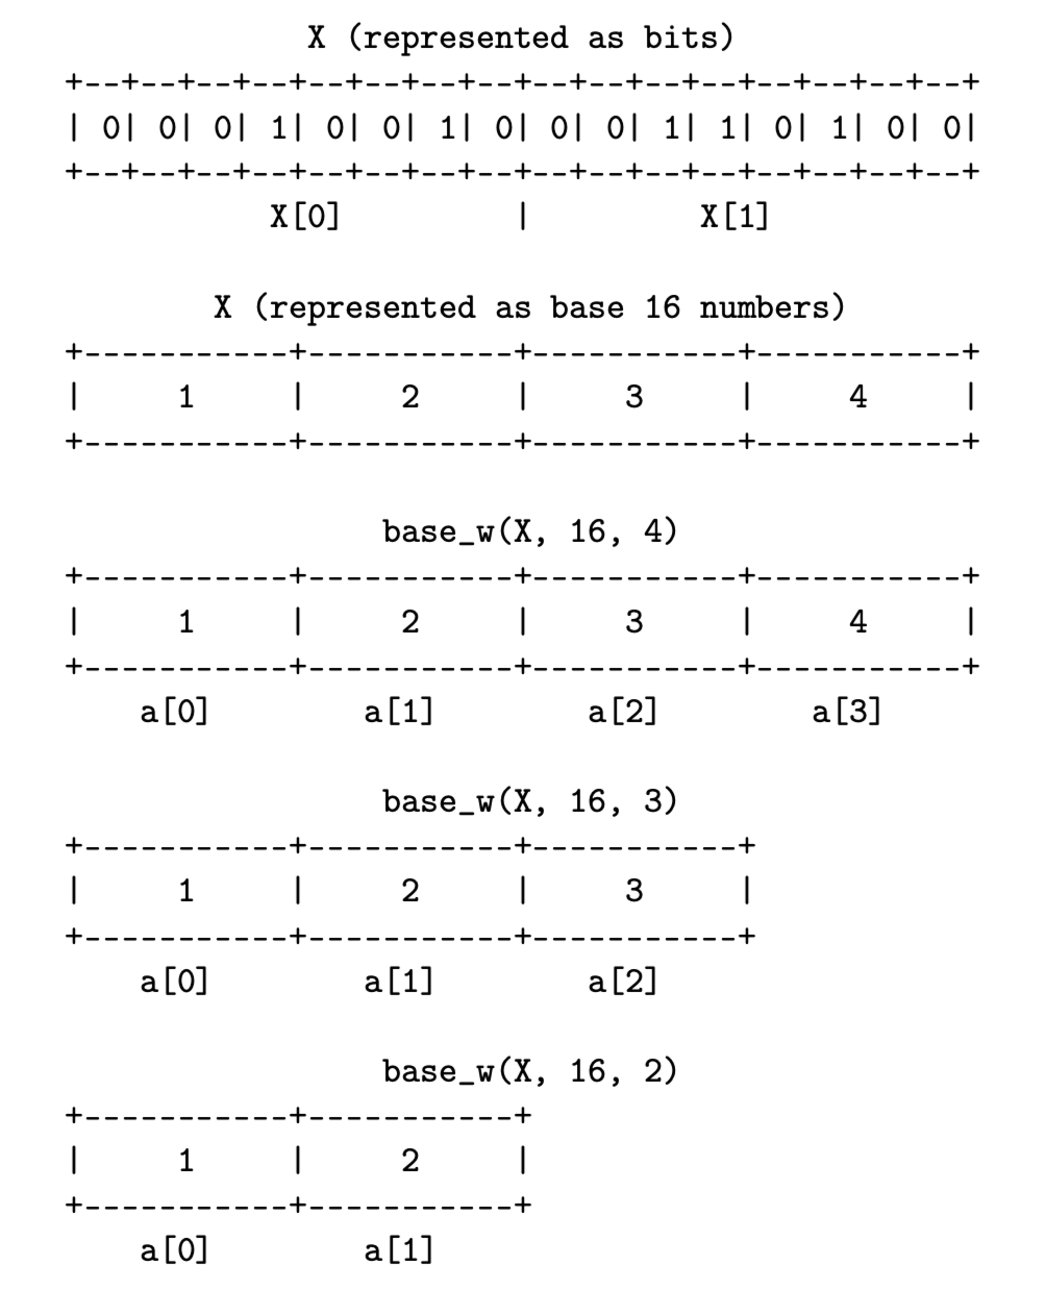
\includegraphics[width=.4\linewidth]{spx-fig/Figure1.pdf}
    \caption{For example, if $X$ is the (big-endian) byte string \texttt{0x1234}, then $\mathtt{base\_w}(X,16,4)$ returns the array $a=\{1,2,3,4\}$.}
    \label{fig:spx1}
\end{figure}
}

The schemes described in this specification build upon several instantiations of tweakable hash functions of the form
\begin{align*}
    \Th_\ell : \byte^n \times \byte^{32} \times \byte^{\ell n} \to \byte^n \\
    \md \gets \Th_\ell (\pk.\seed, \ADRS, M) \enspace,
\end{align*}
mapping and $\ell n$-byte message $M$ to an $n$-byte hash value $md$ using an $n$-byte seed \pk.\seed and a 32-byte address $\ADRS$. The function $\Th_\ell$ is denoted by \texttt{T\_l} in pseudocode.

There are two special cases which we rename for consistency with previous descriptions of hash-based signature schemes:
\begin{align*}
    \hashF& : \byte^{n}\times \byte^{32}\times \byte^{n}\rightarrow \byte^{n} \\
    \hashF& \eqdef \mathbf{T}_1\\
    \hashH& : \byte^{n}\times \byte^{32}\times \byte^{2n}\rightarrow \byte^{n} \\
    \hashH& \eqdef \mathbf{T}_2
\end{align*}

\subsubsection{PRF and Message Digest (Functions \texttt{PRF, PRF\_msg, H\_msg})}

\SPHINCSA\ uses a pseudorandom function \PRF for pseudorandom key generation:

\[\PRF : \byte^{n}\times \byte^{32}\rightarrow \byte^{n} \enspace.\]

In addition, \SPHINCSA\ uses a pseudorandom function $\PRFmsg$ to generate randomness for the message compression:

\[\PRFmsg : \byte^{n}\times \byte^{n}\times \byte^{*}\rightarrow \byte^{n} \enspace.\]

To compress the message to be signed, \SPHINCSA\ uses an additional keyed hash function $\hashmsg$ that can process arbitrary length messages:
\[ \hashmsg : \byte^{n}\times \byte^{n}\times \byte^{n}\times \byte^{*}\rightarrow \byte^{m} \enspace.\]

\subsubsection{Hash Function Address Scheme (Structure of {\ADRS})} \label{sec:addr}

An address \ADRS is a 32-byte value that follows a defined structure. In addition, it comes with set methods to manipulate the address. We explain the generation of addresses in the following sections where they are used. Essentially, all functions have to keep track of the current context, updating the addresses after each hash call.

There are five different types of addresses for the different use cases. One type is used for the hashes in \WOTSCS\ schemes, one is used for compression of the \WOTSCS\ public key, the third is used for hashes within the main Merkle tree construction, another is used for the hashes in the Merkle tree in FORS, and the last is used for the compression of the tree roots of FORS. These types largely share a common format. We describe them in more detail, below.

The structure of an address complies with word borders, with a word being 32 bits long in this context. Only the tree address (i.e. the index of a specific subtree in the main tree) is too long to fit a single word: for this, we reserve three words. An address is structured as follows. It always starts with a layer address of one word in the most significant bits, followed by a tree address of three words. These addresses describe the position of a tree within the hypertree. The layer address describes the height of a tree within the hypertree starting from height zero for trees on the bottom layer. The tree address describes the position of a tree within a layer of a multi-tree starting with index zero for the leftmost tree. The next word defines the type of the address. It is set to 0 for a \WOTSCS\ hash address, to 1 for the compression of the \WOTSCS\ public key, to 2 for a hash tree address, to 3 for a FORS address, and to 4 for the compression of FORS tree roots.

We first describe the \WOTSCS\ address (\cref{fig:spx2}). In this case, the type word is followed by the key pair address that encodes the index of the \WOTSCS\ key pair within the specified tree. The next word encodes the chain address (i.e. the index of the chain within \WOTSCS\ ), followed by a word that encodes the address of the hash function call within the chain. Note that for the generation of the secret keys based on \sk.\seed a different type of address is used (see below).

\begin{figure}[ht]
    \centering
    \begin{bytefield}[bitwidth=1.1em,bitheight=2em]{32}
        \bitbox[lrt]{8}{Layer Address} &
        \bitbox[lrt]{24}{Tree Address} \\ 
        \bitbox{8}{type = 0} & 
        \bitbox{8}{Key Pair Address} &
        \bitbox{8}{Chain Address} &
        \bitbox{8}{Hash Address}
    \end{bytefield} 
    \caption{\WOTSCS\ hash address.}
    \label{fig:spx2}
\end{figure}

The second type (\cref{fig:spx3}) is used to compress the \WOTSCS\ public keys. The type word is set to 1. Similar to the address used within \WOTSCS\ , the next word encodes the key pair address. The remaining two words are not needed, and thus remain zero. We zero pad the address to the constant length of 32 bytes.

\begin{figure}[ht]
    \centering
    \begin{bytefield}[bitwidth=1.1em,bitheight=2em]{32}
        \bitbox[lrt]{8}{Layer Address} &
        \bitbox[lrt]{24}{Tree Address} \\
        \bitbox{8}{type = 1} & 
        \bitbox{8}{Key Pair Address} &
        \bitbox{16}{Padding = 0}
    \end{bytefield}
    \caption{\WOTSCS\ public key compression address.}
    \label{fig:spx3}
\end{figure}

The third type (\cref{fig:spx4}) addresses the hash functions in the main tree. In this case the type word is set to 2, followed by a zero padding of one word. The next word encodes the height of the tree node that is being computed, followed by a word that encodes the index of this node at that height.

\begin{figure}[ht]
    \centering
    \begin{bytefield}[bitwidth=1.1em,bitheight=2em]{32}
        \bitbox[lrt]{8}{Layer Address} &
        \bitbox[lrt]{24}{Tree Address} \\
        \bitbox{8}{type = 2} & 
        \bitbox{8}{Padding = 0} &
        \bitbox{8}{Tree Height} &
        \bitbox{8}{Tree Index}
    \end{bytefield}
    \caption{hash tree address.}
    \label{fig:spx4}
\end{figure}

The next type (\cref{fig:spx5}) is of a similar format, and is used to describe the hash functions in the FORS tree. The type word is set to 3. The key pair address is used to signify which FORS key pair is used, identical to the key pair address in the \WOTSCS\ hash addresses. Its value is the same as that of the \WOTSCS\ key pair that is used to authenticate it, i.e. its index as a leaf in the specified tree. The tree height and tree index fields are used to address the hashes within the FORS tree. This is done like for the above-mentioned hashes in the main tree, with the additional consideration that the tree indices are counted continuously across the different FORS trees. To generate the leaf nodes from \sk.\seed a different type of address is used (see below).

\begin{figure}[ht]
    \centering
    \begin{bytefield}[bitwidth=1.1em,bitheight=2em]{32}
        \bitbox[lrt]{8}{Layer Address} &
        \bitbox[lrt]{24}{Tree Address} \\
        \bitbox{8}{type = 3} & 
        \bitbox{8}{Key Pair Address} &
        \bitbox{8}{Tree Height} &
        \bitbox{8}{Tree Index}
    \end{bytefield}
    \caption{FORS tree address.}
    \label{fig:spx5}
\end{figure}

The next type (\cref{fig:spx6}) is used to compress the tree roots of the FORS trees. The type word is set to 4. Like the \WOTSCS\ public key compression address, it contains only the address of the FORS key pair, but is padded to the full length.

\begin{figure}[ht]
    \centering
    \begin{bytefield}[bitwidth=1.1em,bitheight=2em]{32}
        \bitbox[lrt]{8}{Layer Address} &
        \bitbox[lrt]{24}{Tree Address} \\
        \bitbox{8}{type = 4} & 
        \bitbox{8}{Key Pair Address} &
        \bitbox{16}{Padding = 0}
    \end{bytefield}
    \caption{FORS tree roots compression address.}
    \label{fig:spx6}
\end{figure}


The final two types are used for secret key value generation in \WOTSCS\ and FORS. A \WOTSCS\ key generation address (\cref{fig:spx7}) is the same as a \WOTSCS\ hash address with two differences. First, the type word is set to 5. Second, the hash address word is constantly set to $0$. When generating the secret key value for a given chain, the remaining words have to be set the same way as for the \WOTSCS\ hash addresses used for this chain.

\begin{figure}[ht]
    \centering
    \begin{bytefield}[bitwidth=1.1em,bitheight=2em]{32}
        \bitbox[lrt]{8}{Layer Address} &
        \bitbox[lrt]{24}{Tree Address} \\ 
        \bitbox{8}{type = 5} & 
        \bitbox{8}{Key Pair Address} &
        \bitbox{8}{Chain Address} &
        \bitbox{8}{Hash Address = 0}
    \end{bytefield}
    \caption{\WOTSCS\ key generation address.}
    \label{fig:spx7}
\end{figure}

Similarly, the FORS key generation type (\cref{fig:spx8}) is the same as the FORS tree address type, except that the type word is set to 6, and the tree height word is set to $0$. As for the \WOTSCS\ key generation address, the remaining words have to be set as for the FORS tree address used when processing the generated value.

All fields within these addresses encode unsigned integers. When describing the generation of addresses we use set methods that take positive integers and set the bits of a field to the binary representation of that integer, in big-endian notation. Throughout this document, we adhere to the convention of assuming that changing the type word of an address (indicated by the use of the \texttt{setType()} method) initializes the subsequent three words to zero.

In order to make keeping track of the types easier throughout the pseudo-code in the rest of this document, we refer to them respectively using the constants \verb|WOTS_HASH|, \verb|WOTS_PK|, \verb|TREE|, \verb|FORS_TREE|, \verb|FORS_ROOTS|, \verb|WOTS_PRF|, and \verb|FORS_PRF|.

\begin{figure}[ht]
    \centering
    \begin{bytefield}[bitwidth=1.1em,bitheight=2em]{32}
        \bitbox[lrt]{8}{Layer Address} &
        \bitbox[lrt]{24}{Tree Address} \\
        \bitbox{8}{type = 6} & 
        \bitbox{8}{Key Pair Address} &
        \bitbox{8}{Tree Height = 0} &
        \bitbox{8}{Tree Index}
    \end{bytefield}
    \caption{FORS key generation address.}
    \label{fig:spx8}
\end{figure}

\section{\WOTSCS\ One-Time Signatures} \label{sec:ots}

This section describes the \WOTSCS\ scheme, while a private key can be used to sign any message, each private key MUST NOT
be used to sign more than a single message. 

\subsection{\WOTSCS\ Parameters}
\label{sec:wotspara}
\WOTSCS\ uses the parameters $n,w$ and $\tt len$; They are positive integer values. These parameters are summarized as follows:
\begin{itemize}
    \item $n$: the security parameter; it is the message length as well as the length of a private key, public key, or signature element in bytes.
    \item $w$: the Winternitz parameter;
    \item $\tt len$: the number of $n$-byte-string elements in a \WOTSCS\ private key, public key, and signature.
\end{itemize}

\subsection{\WOTSCS\ Chaining Function (Function {\tt chain})}


The chaining function (Algorithm \ref{alg:chain}) computes an iteration of $\hashF$ on an $n$-byte input using
a \WOTSCS\ hash address \ADRS and a public seed $\pk.\seed$. The address \ADRS MUST
have the first seven 32-bit words set to encode the address of this chain. In each iteration, the address is updated to encode the current position in the chain before \ADRS is used to process the input by $\hashF$.

In the following, \ADRS is a 32-byte \WOTSCS\ hash address as specified in \cref{sec:addr} and $\pk.\seed$ is a $n$-byte string. The chaining function takes as input an $n$-byte string $X$, a start index $i$, a number of steps $s$, as well as \ADRS and $\pk.\seed$. The chaining function returns as output the value obtained by iterating $\hashF$ for $s$ times on input $X$.

\begin{algorithm}
\inputminted[breaklines,linenos,tabsize=2,mathescape,escapeinside=||]{C}{code/chain.cs}
\caption{{\tt chain} --- Chaining function used in \WOTSCS.}
\label{alg:chain}
\end{algorithm}


\subsection{\WOTSCS\ Private Key (Function \texttt{wots\_SKgen})}

The \WOTSCS\ private key, denoted by \sk, is a length $\tt len$ array of $n$-byte strings. This private key MUST NOT be used to sign more than one message. This private key is only implicitly used. Therefore, the following is just to support a better understanding of the following algorithms. Each $n$-byte string in the \WOTSCS\ private key is derived from a secret seed \sk.\seed which is part of the \SPHINCSA\ secret key and a \WOTSCS\ key generation address \texttt{skADRS} using \PRF. The same secret seed is used to generate all secret key values within \SPHINCSA. The address used to generate the $i$-th $n$-byte string of \sk MUST encode the position of the $i$-th hash chain of this \WOTSCS\ instance within the \SPHINCSA\ structure. 

The following pseudocode (Algorithm \ref{alg:wotsskgen}) describes an algorithm to generate a \WOTSCS\ private key.

\begin{algorithm}
\inputminted[breaklines,linenos,tabsize=2,mathescape,escapeinside=||]{C}{code/wots_SKgen.cs}
\caption{\texttt{wots\_SKgen} --- Generating a \WOTSCS\ private key.}
\label{alg:wotsskgen}
\end{algorithm}

\subsection{\WOTSCS\ Public Key Generation (Function \texttt{wots\_PKgen})}

A \WOTSCS\ key pair defines a virtual structure that consists of \len hash chains of length $w.$ Each of the \len stings of $n$-bytes in the private key defines the start node for one hash chain. The public key is the tweakable hash of the end nodes of these hash chains. To compute the hash chains, the chaining function (Algorithm \ref{alg:chain}) is used. A \WOTSCS\ hash address \ADRS and a seed $\pk.\seed$ have to be provided by the calling algorithm as well as a secret seed \sk.\seed. The address \ADRS MUST encode the address of the \WOTSCS\ key pair within the \SPHINCSA\ structure. Hence, a \WOTSCS\ algorithm MUST NOT manipulate any parts of \ADRS other than the last three 32-bit words. Note that the $\pk.\seed$ used here is public information also available to a verifier. 

The following pseudocode (Algorithm \ref{alg:wotspkgen}) describes an algorithm for generating the public key $\pk$.

\begin{algorithm}
\inputminted[breaklines,linenos,tabsize=2,mathescape,escapeinside=||]{C}{code/wots_PKgen.cs}
\caption{\texttt{wots\_PKgen} --- Generating a \WOTSCS\ public key.}
\label{alg:wotspkgen}
\end{algorithm}


\subsection{\WOTSCS\ Encoding (Function \texttt{wots\_encode})}

Let us explain the encoding algorithm (\cref{alg:wotsencode}). The problem can be divided into several subproblems by considering the value of the first element $c_{l-i}$. To encode a natural number $x\in [0,D_{i,m})$, we can simply determine $c_{l-i}=j$ by seeking which $j$ satisfies $x\in [\sum_{k<j}D_{i-1,m-k},\sum_{k\leq j}D_{i-1,m-k})$. Once the value of $v_{l-i}$ is determined, we proceed to its next terms until all elements are decided. All arithmetic operations MUST be compute in unsigned $256$-bit. Array $D$ can be precomputed to avoid computing $D$ for each encoding function call. 

\begin{algorithm}
\inputminted[breaklines,linenos,tabsize=2,mathescape,escapeinside=||]{C}{code/wots_encode.cs}
\caption{\texttt{wots\_encode} --- Encoding message to constant-sum encoding.}
\label{alg:wotsencode}
\end{algorithm}

\subsection{\WOTSCS\ Signature Generation (Function \texttt{wots\_sign})}

A \WOTSCS\ signature is a length $\tt len$ array of $n$-byte strings. The \WOTSCS\ signature is first generated by mapping a message $M$ to $\tt len$ integers between $0$ and $w-1$, and the sum of them is equals to $\lfloor {\tt len}\cdot (w-1)/2 \rfloor$. A \WOTSCS\ hash address \ADRS, a public seed $\pk.\seed$, and a secret seed \sk.\seed have to be provided by the calling algorithm. The address will encode the address of the \WOTSCS\ key pair within a greater structure. Hence, a \WOTSCS\ algorithm MUST NOT manipulate any parts of \ADRS other than the last three 32-bit words. Note that the $\pk.\seed$ used here is public information also available to a verifier while the secret seed \sk.\seed is private information. The pseudocode for generating a \WOTSCS\ signature \sig is shown below (Algorithm \ref{alg:wotssign}).

\begin{algorithm}
\inputminted[breaklines,linenos,tabsize=2,mathescape,escapeinside=||]{C}{code/wots_sign.cs}
\caption{\texttt{wots\_sign} --- Generating a \WOTSCS\ signature on a message $M$.}
\label{alg:wotssign}
\end{algorithm}

The data format for a signature is given in \cref{fig:spx9}.

\begin{figure}[ht]
    \centering
    \begin{bytefield}[bitwidth=1.1em,bitheight=2em]{16}
        \wordbox{1}{$\sigots[0]$} \\
        \wordbox[lrt]{1}{...} \\
        \skippedwords \\
        \wordbox[lrb]{1}{...} \\
        \wordbox{1}{$\sigots[\len-1]$} 
    \end{bytefield}
    %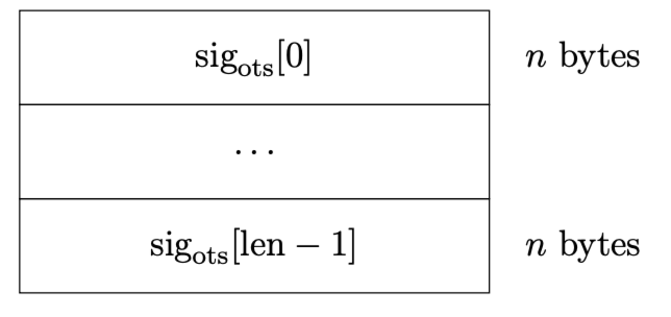
\includegraphics[width=.4\linewidth]{spx-fig/Figure9.pdf}
    \caption{\WOTSCS\ Signature Data Format.}
    \label{fig:spx9}
\end{figure}


\subsection{\WOTSCS\ Compute Public Key from Signature (Function \texttt{wots\_pkFromSig})}

\SPHINCSA\ uses implicit signature verification for \WOTSCS. In order to verify a \WOTSCS\ signature \sig on a message $M$, the verifier computes a \WOTSCS\ public key value from the signature. This can be done by ``completing'' the chain computations starting from the signature values, using the base-w values of the message hash and its checksum. This step, called \texttt{wots\_pkFromSig}, is described below in Algorithm \ref{alg:wotspkfromsig}. The result of \texttt{wots\_pkFromSig} then has to be verified. In a standalone version, this would be done by simple comparison. When used in \SPHINCSA\ the output value is verified by using it to compute a \SPHINCSA\ public key. 

A \WOTSCS\ hash address \ADRS and a public seed $\pk.\seed$ have to be provided by the calling algorithm. The address will encode the address of the \WOTSCS\ key pair within the \SPHINCSA\ structure. Hence, a \WOTSCS\ algorithm MUST NOT manipulate any parts of \ADRS other than the last three 32-bit words. Note that the $\pk.\seed$ used here is public information also available to a verifier.

\begin{algorithm}
\inputminted[breaklines,linenos,tabsize=2,mathescape,escapeinside=||]{C}{code/wots_pkFromSig.cs}
\caption{\texttt{wots\_pkFromSig} --- Computing a \WOTSCS\ public key from a message and its signature.}
\label{alg:wotspkfromsig}
\end{algorithm}


\section{The \SPHINCSA\ Hypertree}

In this section, we explain how the \SPHINCSA\ hypertree is built. We first explain how \WOTSCS\ gets combined with a binary hash tree, leading to a fixed input-length version of the eXtended Merkle Signature Scheme (XMSS). Afterwards, we explain how to go to a hypertree from there. The hypertree might be viewed as a fixed input-length version of multi-tree XMSS (\XMSSMT).


\subsection{(Fixed Input-Length) XMSS} \label{sec:xmss}

XMSS is a method for signing a potentially large but fixed number of messages. It is based on the Merkle signature scheme. It authenticates $2^{h'}$ $\WOTSCS$ public keys using a binary tree of height $h'$. Hence, an XMSS key pair for height $h'$ can be used to sign 2 different messages. Each node in the binary tree is an $n$-byte value which is the tweakable hash of the concatenation of its two child nodes. The leaves are the \WOTSCS\ public keys. The XMSS public key is the root node of the tree. In \SPHINCSA, the XMSS secret key is the single secret seed that is used to generate all \WOTSCS\ secret keys.

An XMSS signature in the context of \SPHINCSA\ consists of the \WOTSCS\ signature on the message and the so-called authentication path. The latter is a vector of tree nodes that allow a verifier to compute a value for the root of the tree starting from a \WOTSCS\ signature. A verifier computes the root value and verifies its correctness. A standalone XMSS signature also contains the index of the used \WOTSCS\ key pair. In the context of \SPHINCSA\ this is not necessary as the \SPHINCSA\ signature allows to compute the index for each XMSS signature contained.

\subsubsection{XMSS Parameters}
\label{sec:xmsspara}
XMSS has the following parameters:

\begin{itemize}
    \item $h'$ : the height ($\text{number of levels} - 1$) of the tree.

    \item $n$: the length in bytes of messages as well as of each node.

    \item $w$ : the Winternitz parameter as defined for \WOTSCS\ in the previous Section.
\end{itemize}

There are $2^{h'}$ leaves in the tree. XMSS signatures are denoted by \sigxmss  (\texttt{SIG\_XMSS} in pseudocode). \WOTSCS\ signatures are denoted by \sig.

XMSS parameters are implicitly included in algorithm inputs as needed.

\subsubsection{XMSS Private Key}

In the context of \SPHINCSA, an XMSS private key is the single secret seed \sk.\seed contained in the \SPHINCSA\ secret key. It is used to generate the \WOTSCS\ secret keys within the structure of an XMSS key pair as described in \cref{sec:ots}.

\subsubsection{TreeHash (Function \texttt{treehash})}

For the computation of the internal $n$-byte nodes of a Merkle tree, the subroutine \texttt{treehash} (\cref{alg:treehash}) accepts a secret seed \sk.\seed, a public seed $\pk.\seed$, an unsigned integer $s$ (the start index), an unsigned integer $z$ (the target node height), and an address \ADRS that encodes the address of the containing tree. For the height of a node within a tree, counting starts with the leaves at height zero. The \texttt{treehash} algorithm returns the root node of a tree of height $z$ with the leftmost leaf being the \WOTSCS\ pk at index $s$. It is REQUIRED that $s$ \% $2^{z}=0$, i.e. that the leaf at index $s$ is a leftmost leaf of a sub-tree of height $z$. Otherwise the algorithm fails as it would compute non-existent nodes. The \texttt{treehash} algorithm described here uses a stack holding up to $(z-1)$ nodes, with the usual stack functions \texttt{push()} and \texttt{pop()}. We furthermore assume that the height of a node (an unsigned integer) is stored alongside a node's value (an $n$-byte string) on the stack.

\begin{algorithm}
\inputminted[breaklines,linenos,tabsize=2,mathescape,escapeinside=||]{C}{code/treehash.cs}
\caption{\texttt{treehash} --- The TreeHash algorithm.}
\label{alg:treehash}
\end{algorithm}

\subsubsection{XMSS Public Key Generation (Function \texttt{xmss\_PKgen})}

The XMSS public key is computed as described in \texttt{xmss\_PKgen} (\cref{alg:xmsspkgen}). In the context of \SPHINCSA\ the XMSS public key PK is the root of the binary hash tree. The root is computed using \texttt{treehash}. The public key generation takes a secret seed \sk.\seed, a public seed \pk.\seed, and an address \ADRS. The latter encodes the position of this XMSS instance within the \SPHINCSA\ structure.

\begin{algorithm}
    \inputminted[breaklines,linenos,tabsize=2,mathescape,escapeinside=||]{C}{code/xmss_PKgen.cs}
    \caption{\texttt{xmss\_PKgen} --- Generating an XMSS public key.}
    \label{alg:xmsspkgen}
\end{algorithm}

\subsubsection{XMSS Signature}

An XMSS signature is a $((\len+h')*n)$-byte string consisting of
\begin{itemize}
    \item a \WOTSCS\ signature \sigots taking $\len\cdot n$ bytes,

    \item the authentication path \texttt{AUTH} for the leaf associated with the used \WOTSCS\ key pair taking $h'\cdot n$ bytes.
\end{itemize}

The authentication path is an array of $h'$ $n$-byte strings. It contains the siblings of the nodes in on the path from the used leaf to the root. It does not contain the nodes on the path itself. These nodes in \texttt{AUTH} are needed by a verifier to compute a root node for the tree from a \WOTSCS\ public key. A node $N$ is addressed by its position in the tree. $N(x, y)$ denotes the $y$-th node on level $x$ with $y=0$ being the leftmost node on a level. The leaves are on level $0$, the root is on level $h'$. An authentication path contains exactly one node on every layer $0\leq x\leq(h'-1)$ . For the $i$-th $\WOTSCS$ key pair, counting from zero, the $j$-th authentication path node is
\[ \mathtt{AUTH}[j]=N\left(j, \lfloor\frac{i}{2^{j}}\rfloor\oplus 1\right) \enspace.\]

The computation of the authentication path is discussed in \cref{sec:xmsssign}. The data format for a signature is given in \cref{fig:spx10}.

\begin{figure}[ht]
    \centering
    \begin{bytefield}[bitwidth=1.1em,bitheight=2em]{16}
        \wordbox{2}{$\mathbf{sig}$} \\
        \wordbox{1}{$\mathbf{AUTH}[0]$} \\
        \wordbox[lrt]{1}{...} \\
        \skippedwords \\
        \wordbox[lrb]{1}{...} \\
        \wordbox{1}{$\mathbf{AUTH}[h-1]$}
    \end{bytefield}
    %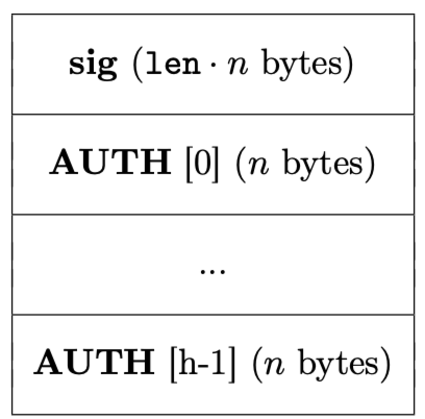
\includegraphics[width=.4\linewidth]{spx-fig/Figure10.pdf}
    \caption{XMSS Signature} \label{fig:spx10}
\end{figure}

\subsubsection{XMSS Signature Generation (Function \texttt{xmss\_sign})}
\label{sec:xmsssign}

To compute the XMSS signature of a message $M$ in the context of \SPHINCSA, the secret seed \sk.\seed, the public seed $\pk.\seed$, the index \texttt{idx} of the \WOTSCS\ key pair to be used, and the address \ADRS of the XMSS instance are needed. First, a \WOTSCS\ signature of the message digest is computed using the \WOTSCS\ instance at index \texttt{idx}. Next, the authentication path is computed.

The node values of the authentication path MAY be computed in any way. The least memory-intensive method is to compute all nodes using the \texttt{treehash} algorithm (\cref{alg:treehash}). This is described here. Note that the details of how this step is implemented are not relevant to interoperability; it is not necessary to know any of these details in order to perform the signature verification operation.

\begin{algorithm}
\inputminted[breaklines,linenos,tabsize=2,mathescape,escapeinside=||]{C}{code/xmss_sign.cs}
\caption{\texttt{xmss\_sign} --- Generating an XMSS signature.}
\label{alg:xmsssign}
\end{algorithm}

\subsubsection{XMSS Compute Public Key from Signature (Function \texttt{xmss\_pkFromSig})}

\SPHINCSA\ makes use of implicit signature verification of XMSS signatures. An XMSS signature is used to compute a candidate XMSS public key, i.e., the root of the tree. This is used in further computations (signature of the tree above) and implicitly verified by the outcome of that computation. Hence, this specification does not contain an \texttt{xmss\_verify} method but the method \texttt{xmss\_pkFromSig}.

The method \texttt{xmss\_pkFromSig} takes an $n$-byte message $M$, an XMSS signature \sigxmss, a signature index \texttt{idx}, a public seed $\pk.\seed$, and an address $\ADRS$. The latter encodes the position of the current XMSS instance within the virtual structure of the \SPHINCSA\ key pair. First, \texttt{wots\_pkFromSig} is used to compute a candidate \WOTSCS\ public key. This in turn is used together with the authentication path to compute a root node which is then returned. The algorithm \texttt{xmss\_pkFromSig} is given as \cref{alg:xmsspkfromsig}.

\begin{algorithm}
\inputminted[breaklines,linenos,tabsize=2,mathescape,escapeinside=||]{C}{code/xmss_pkFromSig.cs}
\caption{\texttt{xmss\_pkFromSig} --- Computing an XMSS public key from an XMSS signature.}
\label{alg:xmsspkfromsig}
\end{algorithm}




\subsection{HT: The Hypertree}

The \SPHINCSA\ hypertree HT is a variant of \XMSSMT. It is essentially a certification tree of XMSS instances. A HT is a tree of several layers of XMSS trees. The trees on top and intermediate layers are used to sign the public keys, i.e., the root nodes, of the XMSS trees on the respective next layer below. Trees on the lowest layer are used to sign the actual messages, which are FORS public keys in \SPHINCSA. All XMSS trees in HT have equal height.

Consider a HT of total height $h$ that has $d$ layers of XMSS trees of height $h'=h/d$. Then layer $d-1$ contains one XMSS tree, layer $d-2$ contains $2^{h'}$ XMSS trees, and so on. Finally, layer $0$ contains $2^{h-h'}$ XMSS trees.

\subsubsection{HT Parameters}
\label{sec:htpara}
In addition to all XMSS parameters, a HT requires the hypertree height $h$ and the number of tree layers $d$, specified as an integer value that divides $h$ without remainder. The same tree height $h'=h/d$ and the same Winternitz parameter $w$ are used for all tree layers.


\subsubsection{HT Key Generation (Function \texttt{ht\_PKgen})}

The HT private key is the secret seed \sk.\seed which is used to generate all the \WOTSCS\ private keys within the virtual structure spanned by the HT.

The HT public key is the public key (root node) of the single XMSS tree on the top layer. Its computation is explained below. The public key generation takes as input a private and a public seed.

\begin{algorithm}
\inputminted[breaklines,linenos,tabsize=2,mathescape,escapeinside=||]{C}{code/ht_PKgen.cs}
\caption{\texttt{ht\_PKgen} --- Generating an HT public key.}
\label{alg:htpkgen}
\end{algorithm}
\subsubsection{HT Signature}

A HT signature $\sight$ is a byte string of length $(h+d*\len)*n$. It consists of $d$ XMSS signatures (of $(h/d+\len)*n$ bytes each).

The data format for a signature is given in \cref{fig:spx11}.

\begin{figure}[ht]
    \centering
    \begin{bytefield}[bitwidth=1.1em,bitheight=2em]{16}
        \wordbox{1}{XMSS Signature $\mathbf{sig}_{\XMSS}$} \\
        \wordbox{1}{$\mathbf{AUTH}[0]$} \\
        \wordbox[lrt]{1}{...} \\
        \skippedwords \\
        \wordbox[lrb]{1}{...} \\
        \wordbox{1}{$\mathbf{AUTH}[h-1]$}
    \end{bytefield}
    %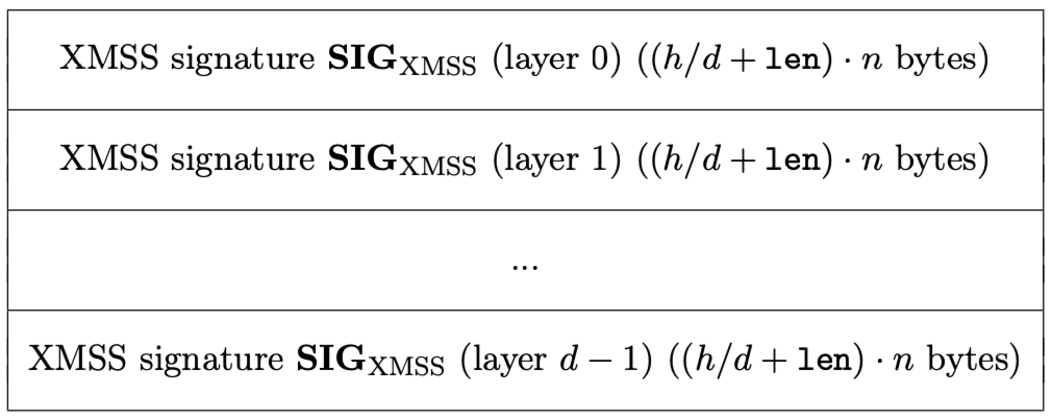
\includegraphics[width=.4\linewidth]{spx-fig/Figure11.pdf}
    \caption{HT Signature.} \label{fig:spx11}
\end{figure}

\subsubsection{HT Signature Generation (Function \texttt{ht\_sign})}

To compute a HT signature $\sight$ of a message $M$ using, \texttt{ht\_sign} (\cref{alg:htsign}) described below uses \texttt{xmss\_sign} as defined in \cref{sec:xmsssign}. The algorithm \texttt{ht\_sign} takes as input a message $M$, a private seed \sk.\seed, a public seed $\pk.\seed$, and an index \texttt{idx}. The index identifies the leaf of the hypertree to be used to sign the message. The HT signature then consists of a stack of XMSS signatures using the XMSS trees on the path from the leaf with index idx to the top tree. Note that idx is passed as two separate arguments, split into an index to address the specific tree and the leaf index within that tree. This allows for a somewhat higher hypertree, as one can use a 64-bit integer for \texttt{tree\_idx} to support parameters that conform to $h<64+h/d$. This matches the parameters in this specification If other parameter sets are used that allow greater $h$, the data type of \texttt{tree\_idx} MUST be adapted accordingly.

Algorithm \texttt{ht\_sign} uses \texttt{xmss\_pkFromSig} to compute the root node of an XMSS instance after that instance was used for signing. An alternative is to use \texttt{xmss\_PKgen}. However, \texttt{xmss\_PKgen} rebuilds the whole tree while \texttt{xmss\_pkFromSig} only does one call to \texttt{wots\_pkFromSig} and $(h'-1)$ calls to $\hashH$. The algorithm \texttt{ht\_sign} as described below is just one way to generate a HT signature. Other methods MAY be used as long as they generate the same output.

\begin{algorithm}
    \inputminted[breaklines,linenos,tabsize=2,mathescape,escapeinside=||]{C}{code/ht_sign.cs}
    \caption{\texttt{ht\_sign} --- Generating an HT signature.}
    \label{alg:htsign}
\end{algorithm}

\subsubsection{HT Signature Verification (Function \texttt{ht\_verify})}

HT signature verification (\cref{alg:htverify}) can be summarized as $d$ calls to \texttt{xmss\_pkFromSig} and one comparison with a given value. HT signature verification takes a message $M$, a signature $\sight$, a public seed $\pk.\seed$, an index \texttt{idx} (split into a tree index and a leaf index, as above), and a HT public key $\pk_{\mathtt{HT}}.$

\begin{algorithm}
    \inputminted[breaklines,linenos,tabsize=2,mathescape,escapeinside=||]{C}{code/ht_verify.cs}
    \caption{\texttt{ht\_verify} --- Verifying a HT signature $\bf {SIG}_{HT}$ on a message $M$ using a HT public key ${\bf PK}_{HT}$.}
    \label{alg:htverify}
\end{algorithm}
\section{FORS: Forest Of Random Subsets}

The \SPHINCSA\ hypertree HT is not used to sign the actual messages but the public keys of FORS instances which in turn are used to sign message digests. FORS, short for forest of random subsets, is a few-time signature scheme (FTS). FORS is an improvement of HORST \cite{EC:BHHLNP15} which in turn is a variant of HORS \cite{EPRINT:ReyRey02}. For security it is essential that the input to FORS is the output of a hash function. In the following we describe FORS as acting on bit strings.

FORS uses parameters $k$ and $t=2^{a}$ (example parameters are $t=2^{15}, k=10$). FORS signs strings of length $ka$ bits. Here, we deviate from defining sizes in bytes as the message length in bits might not be a multiple of eight. The private key consists of $kt$ random {\it n}- byte strings grouped into $k$ sets, each containing $t n$-byte strings. The private key values are pseudorandomly generated from the main private seed \sk.\seed in the \SPHINCSA\ private key. In \SPHINCSA, the FORS private key values are only temporarily generated as an intermediate result when computing the public key or a signature.

The FORS public key is a single $n$-byte hash value. It is computed as the tweakable hash of the root nodes of $k$ binary hash trees. Each of these binary hash trees has height $a$ and is used to authenticate the $t$ private key values of one of the $k$ sets. Accordingly, the leaves of a tree are the (tweakable) hashes of the values in its private key set.

A signature on a string $M$ consists of $k$ private key values --- one per set of private key elements --- and the associated authentication paths. To compute the signature, $\md$ is split into $k$ a-bit strings. As \md is a sequence of bytes, we first convert to a bit-string by enumerating the bytes in $\md$, internally enumerating the bits within a byte from least to most significant. Next, each of these bit strings is interpreted as an integer between $0$ and $t-1$. Each of these integers is used to select one private key value from a set. I.e., if the first integer is $i$, the $i$-th private key element of the first set gets selected and so on. The signature consists of the selected private key elements and the associated authentication paths.

\SPHINCSA\ uses implicit verification for FORS, only using a method to compute a candidate public key from a signature. This is done by computing root nodes of the $k$ trees using the indices computed from the input string as well as the private key values and authentication paths form the signature. The tweakable hash of these roots is then returned as candidate public key.

We now describe the parameters and algorithms for FORS.

\subsection{FORS Parameters}
\label{sec:forspara}
FORS uses the parameters $n, k$, and $t$; they all take positive integer values. These parameters are summarized as follows:

\begin{itemize}
    \item $ n$: the security parameter; it is the length of a private key, public key, or signature element in bytes.

    \item $ k$: the number of private key sets, trees and indices computed from the input string.
    
    \item $ t$: the number of elements per private key set, number of leaves per hash tree and upper bound on the index values. The parameter $t$ MUST be a power of 2. If $t=2^{a}$, then the trees have height $a$ and the input string is split into bit strings of length $a.$
\end{itemize}


Inputs to FORS are bit strings of length $k\log t.$

\begin{figure}[ht]
    \centering
    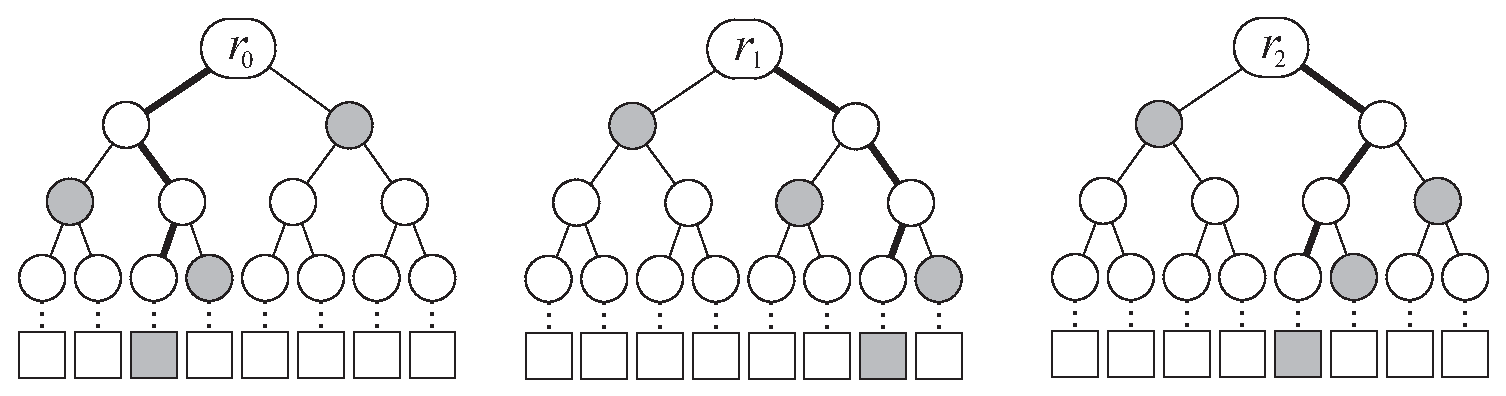
\includegraphics[width=.8\linewidth]{figure/fors.eps}
    %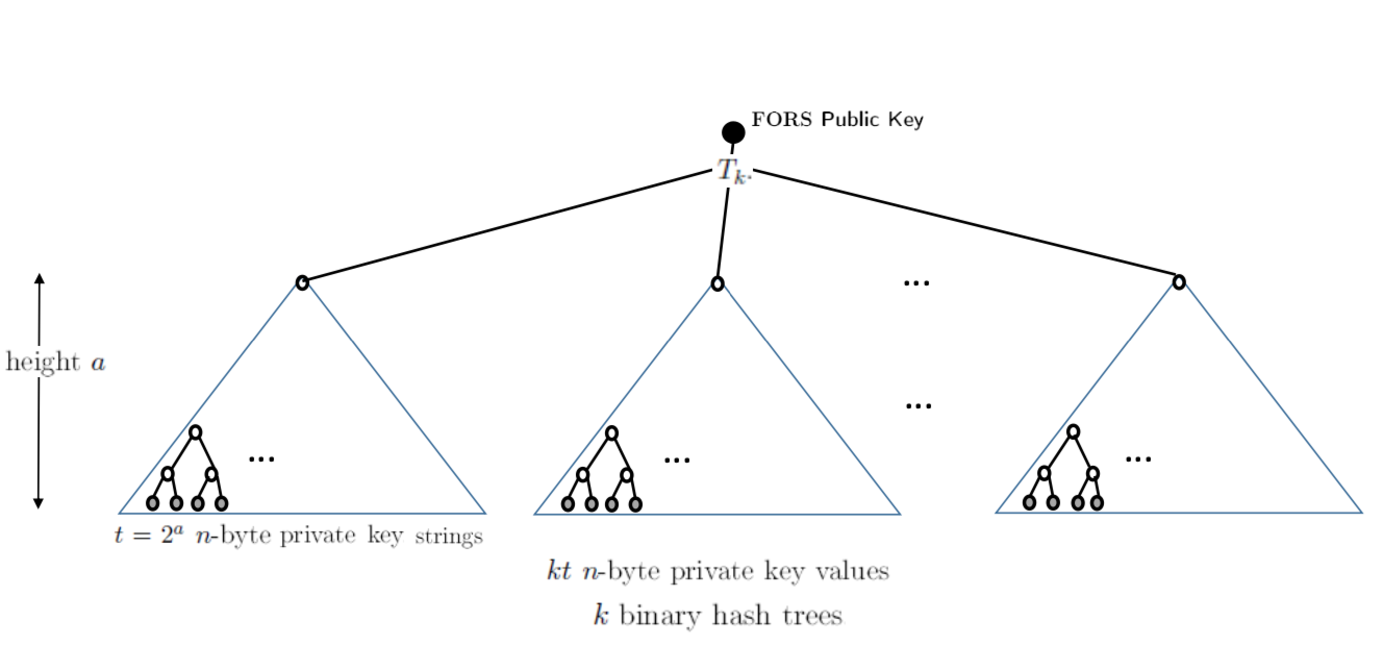
\includegraphics[width=.8\linewidth]{spx-fig/Figure12.pdf}
    \caption{FORS trees and PK.} \label{fig:spx12}
\end{figure}

\subsection{FORS Private Key (Function \texttt{fors\_SKgen})}

In the context of \SPHINCSA, a FORS private key is the single private seed \sk.\seed contained in the \SPHINCSA\ private key. It is used to generate the $kt$ $n$-byte private key values using \PRF with a FORS key generation address. While these values are logically grouped into a two-dimensional array, for implementations it makes sense to assume they are in a one dimensional array of length $kt$. The jth element of the $i$-th set is then stored at $\sk[it+j].$ To generate one of these elements, a FORS key generation address skADRS is used, that encodes the position of the FORS key pair within \SPHINCSA\ and has tree height set to $0$ and leaf index set to $it+j$:

\begin{algorithm}
    \inputminted[breaklines,linenos,tabsize=2,mathescape,escapeinside=||]{C}{code/fors_SKgen.cs}
    \caption{\texttt{fors\_SKgen} --- Computing a FORS private key value.}
    \label{alg:forsskgen}
\end{algorithm}

\subsection{FORS TreeHash (Function \texttt{fors\_treehash})}

Before coming to the FORS public key, we have to discuss computation of the trees. For the computation of the $n$-byte nodes in the FORS hash trees, the subroutine \texttt{fors\_treehash} is used. It is essentially the same algorithm as \texttt{treehash} (\cref{alg:treehash}) in \cref{sec:xmss}. The two differences are how the leaf nodes are computed and how addresses are handled. However, as the addresses are similar, an implementation can implement both algorithms in the same routine easily.

Algorithm \texttt{fors\_treehash} accepts a secret seed \sk.\seed, a public seed $\pk.\seed$, an unsigned integer $s$ (the start index), an unsigned integer $z$ (the target node height), and an address \ADRS that encodes the address of the FORS key pair. As for \texttt{treehash}, the \texttt{fors\_treehash} algorithm returns the root node of a tree of height $z$ with the leftmost leaf being the hash of the private key element at index $s$. Here, $s$ is ranging over the whole $kt$ private key elements. It is REQUIRED that $s$ \% $2^{z}=0$, i.e. that the leaf at index $s$ is a leftmost leaf of a sub-tree of height $z$. Otherwise the algorithm fails as it would compute non-existent nodes.

\begin{algorithm}
    \inputminted[breaklines,linenos,tabsize=2,mathescape,escapeinside=||]{C}{code/fors_treehash.cs}
    \caption{The \texttt{fors\_treehash algorithm.}}
    \label{alg:forstreehash}
\end{algorithm}

\subsection{FORS Public Key (Function \texttt{fors\_PKgen})}

In the context of \SPHINCSA, the FORS public key is never generated alone. It is only generated together with a signature. We include \texttt{fors\_PKgen} for completeness, a better understanding, and testing. Algorithm \texttt{fors\_PKgen} takes a private seed \sk.\seed, a public seed $\pk.\seed$, and a FORS address \ADRS. The latter encodes the position of the FORS instance within \SPHINCSA. It outputs a FORS public key.

\begin{algorithm}
    \inputminted[breaklines,linenos,tabsize=2,mathescape,escapeinside=||]{C}{code/fors_PKgen.cs}
    \caption{\texttt{ fors\_PKgen } --- Generate a FORS public key. }
    \label{alg:forspkgen}
\end{algorithm}


\subsection{FORS Signature Generation (Function \texttt{fors\_sign})}

A FORS signature is a length $k(\log t+1)$ array of $n$-byte strings. It contains $k$ private key values, $n$-bytes each, and their associated authentication paths, $\log t$ $n$-byte values each.

The algorithm \texttt{fors\_sign} takes a $(k\log t)$-bit string $M$, a private seed \sk.\seed, a public seed $\pk.\seed$, and an address \ADRS. The latter encodes the position of the FORS instance within \SPHINCSA. It outputs a FORS signature $\sigfors$.

\begin{algorithm}
    \inputminted[breaklines,linenos,tabsize=2,mathescape,escapeinside=||]{C}{code/fors_sign.cs}
    \caption{\texttt{ fors\_sign } --- Generate a FORS signature on string $M$. }
    \label{alg:forssign}
\end{algorithm}

The data format for a signature is given in \cref{fig:spx13}.

\begin{figure}[ht]
    \centering
    \begin{bytefield}[bitwidth=1.1em,bitheight=2em]{16}
        \wordbox{1}{Private Key Value (Tree 0)} \\
        \wordbox{1}{$\mathbf{AUTH}$ (Tree 0)} \\
        \wordbox[lrt]{1}{...} \\
        \skippedwords \\
        \wordbox[lrb]{1}{...} \\
        \wordbox{1}{Private Key Value (Tree $k-1$)} \\
        \wordbox{1}{$\mathbf{AUTH}$ (Tree $k-1$)} \\
    \end{bytefield}
    %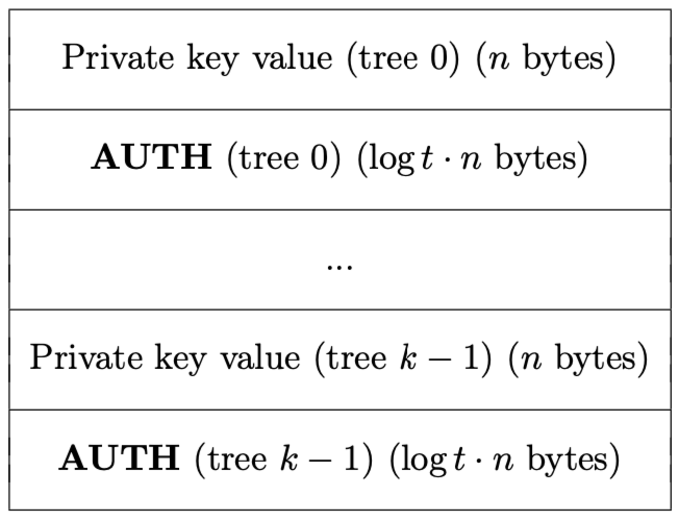
\includegraphics[width=.4\linewidth]{spx-fig/Figure13.pdf}
    \caption{FORS Signature.} \label{fig:spx13}
\end{figure}

\subsection{FORS Compute Public Key from Signature (Function \texttt{fors\_pkFromSig})}

\SPHINCSA\ makes use of implicit signature verification of FORS signatures. A FORS signature is used to compute a candidate FORS public key. This public key is used in further computations (message for the signature of the XMSS tree above) and implicitly verified by the outcome of that computation. Hence, this specification does not contain a \texttt{fors\_verify} method but the method \texttt{fors\_pkFromSig}.

The method \texttt{fors\_pkFromSig} takes a $ k\log t$-bit string $M$, a FORS signature $\sigfors$, a public seed \pk.\seed, and an address \ADRS. The latter encodes the position of the FORS instance within the virtual structure of the \SPHINCSA\ key pair. First, the roots of the $k$ binary hash trees are computed using \texttt{fors\_treehash}. Afterwards the roots are hashed using the tweakable hash function $\mathrm{T}_{k}$. The algorithm \texttt{fors\_pkFromSig} is given as \cref{alg:forspkfromsig}. The method \texttt{fors\_pkFromSig} makes use of functions \sigfors.\texttt{getSK(i)} and \sigfors.\texttt{getAUTH(i)}. The former returns the $i$-th secret key element stored in the signature, the latter returns the $i$-th authentication path stored in the signature.

\begin{algorithm}
    \inputminted[breaklines,linenos,tabsize=2,mathescape,escapeinside=||]{C}{code/fors_pkFromSig.cs}
    \caption{\texttt{ fors\_pkFromSig } --- Compute a FORS public key from a FORS signature. }
    \label{alg:forspkfromsig}
\end{algorithm}

\section{\SPHINCSA}
We now have all ingredients to describe our main construction \SPHINCSA. Essentially, \SPHINCSA\ follows the fundamental structure of \SPHINCSA\ with the only difference being the one-time signature component.

\subsection{\SPHINCSA\ Parameters}

\SPHINCSA\ has the following parameters:

\begin{itemize}

    \item $n$: the security parameter in bytes.

    \item $w$: the Winternitz parameter as defined in Section \ref{sec:wotspara}.
    
    \item $h$: the height of the hypertree as defined in Section \ref{sec:htpara}.
    
    \item $d$: the number of layers in the hypertree as defined in Section \ref{sec:htpara}.
    
    \item $k$: the number of trees in FORS as defined in Section \ref{sec:forspara}.
    
    \item $t$: the number of leaves of a FORS tree as defined in Section \ref{sec:forspara}.
    
\end{itemize}

All the restrictions stated in the previous sections apply. Recall that we use $a=\log t.$ Moreover, from these values the values $m$ and \len are computed as

\begin{itemize}
    \item $m$: the message digest length in bytes. It is computed as
    $$
    m=\lfloor(k\log t+7)/8\rfloor+\lfloor(h-h/d+7)/8\rfloor+\lfloor(h/d+7)/8\rfloor.
    $$
    While only $h+k\log t$ bits would be needed, using the longer $m$ as defined above simplifies implementations significantly.
    
    \item $\len$: the number of $n$-byte string elements in a \WOTSCS\ private key, public key, and signature. The value $\len$ is chosen so that the size of the following poset is larger than the desired message space $\bool^n$ (cf.~\cref{sec:balanced wotsp}).
    \[\left| D_{ \len, \lfloor \frac{\len \cdot (w-1)}{2} \rfloor } \right| \geq 2^n \enspace. \]

\end{itemize}
In the following, we assume that all algorithms have access to these parameters.

\subsection{\SPHINCSA\ Key Generation (Function \texttt{spx\_keygen})}

The \SPHINCSA\ private key contains two elements. First, the $n$-byte secret seed $\sk.\seed$ which is used to generate all the \WOTSCS\ and FORS private key elements. Second, an $n$-byte PRF key $\sk.\prf$ which is used to deterministically generate a randomization value for the randomized message hash.

The \SPHINCSA\ public key also contains two elements. First, the HT public key, i.e.~the root of the tree on the top layer. Second, an $n$-byte public seed value $\pk.\seed$ which is sampled uniformly at random.

As \texttt{spa\_sign} does not get the public key, but needs access to $\pk.\seed$ (and possibly to $\pk.\root$ for fault attack mitigation), the \SPHINCSA\ secret key contains a copy of the public key.

The description of algorithm \texttt{spa\_keygen} assumes the existence of a function \texttt{sec\_rand} which on input $i$ returns $i$-bytes of cryptographically strong randomness.

\begin{algorithm}
    \inputminted[breaklines,linenos,tabsize=2,mathescape,escapeinside=||]{C}{code/spa_keygen.cs}
    \caption{\texttt{spa\_keygen} ---  Generate a \SPHINCSA\ key pair.}
    \label{alg:spxkeygen}
\end{algorithm}

The format of a \SPHINCSA\ private and public key is given in \cref{fig:spx14}.

\begin{figure}[ht]
    \centering
    \begin{bytefield}[bitwidth=1.1em,bitheight=2em]{8}
        \wordbox{1}{$\sk.\mathtt{seed}$} \\
        \wordbox{1}{$\sk.\mathtt{prf}$} \\
        \wordbox{1}{$\pk.\mathtt{seed}$} \\
        \wordbox{1}{$\pk.\mathtt{root}$}
    \end{bytefield}
    \qquad
    \begin{bytefield}[bitwidth=1.1em,bitheight=2em]{8}
        \wordbox{1}{$\pk.\mathtt{seed}$} \\
        \wordbox{1}{$\pk.\mathtt{root}$}
    \end{bytefield} 

    %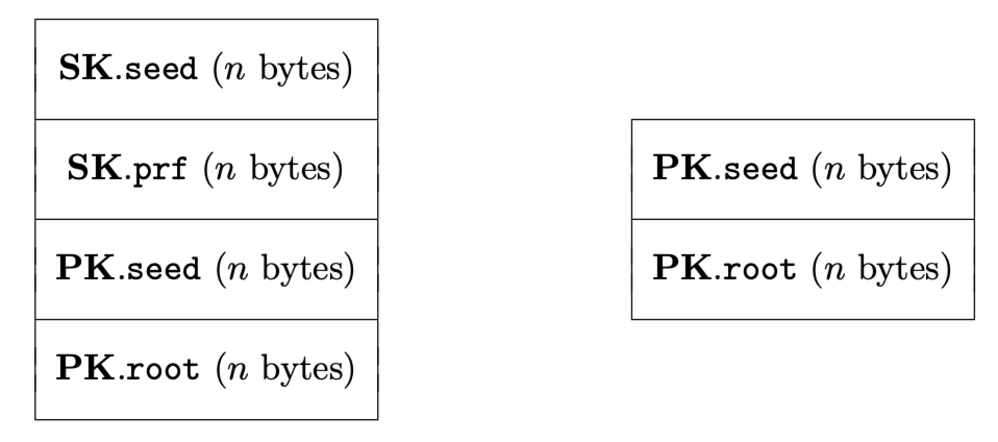
\includegraphics[width=.8\linewidth]{spx-fig/Figure14.pdf}
    \caption{Left: \SPHINCSA\ secret key. Right: \SPHINCSA\ public key.} \label{fig:spx14}
\end{figure}

\subsection{\SPHINCSA\ Signature}

A \SPHINCSA\ signature $\sight$ is a byte string of length $(1 + k \cdot (a+1) + h + d \cdot \len)n$. It consists of an $n$-byte randomization string \randstr, a FORS signature $\sigfors$ consisting of $k(a+1)n$-byte strings, and a HT signature $\sight$ of $(h + d \cdot \len)n$ bytes.

The data format for a signature is given in \cref{fig:spx15}.

\begin{figure}[ht]
    \centering
    \begin{bytefield}[bitwidth=1.1em,bitheight=2em]{16}
        \wordbox{1}{Randomness $\randstr$} \\
        \wordbox{1}{FORS Signature $\sigfors$} \\
        \wordbox{1}{HT Signature $\sight$}
    \end{bytefield} 
    %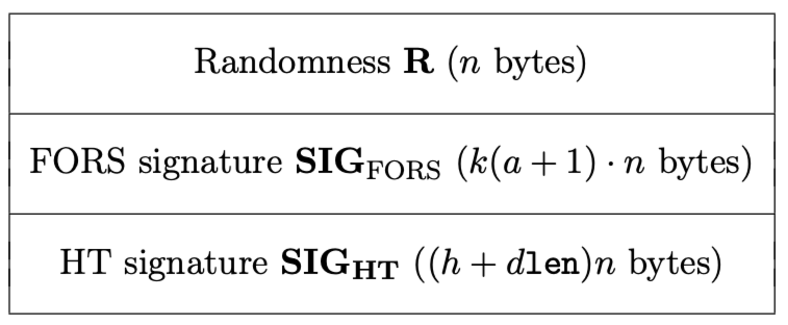
\includegraphics[width=.4\linewidth]{spx-fig/Figure15.pdf}
    \caption{ \SPHINCSA\ signature.} \label{fig:spx15}
\end{figure}

\subsection{\SPHINCSA\ Signature Generation (Function \texttt{spa\_sign})}

Generating a \SPHINCSA\ signature consists of four steps. First, a random value $\randstr$ is pseudorandomly generated. Next, this is used to compute a $m$ byte message digest which is split into a $\lfloor(k\log t+7)/8\rfloor$-byte partial message digest \texttt{tmp\_md}, a $\lfloor(h-h/d+7)/8\rfloor$-byte tree index \texttt{tmp\_idx\_tree}, and a $\lfloor(h/d+7)/8\rfloor$-byte leaf index \texttt{tmp\_idx\_leaf}. Next, the actual values $\md$, \texttt{idx\_tree}, and \texttt{idx\_leaf} are computed by extracting the necessary number of bits. The partial message digest md is then signed with the \texttt{idx\_leaf}-th FORS key pair of the \texttt{idx\_tree}-th XMSS tree on the lowest HT layer. The public key of the FORS key pair is then signed using HT.The index is never actually used as a whole, but immediately split into a tree index and a leaf index, for ease of implementation. 

When computing $\tt{R}$, the PRF takes a $n$-byte string opt which is initialized with $\pk.\seed$ but can be overwritten with randomness if the global variable \texttt{RANDOMIZE} is set. This option is given as otherwise \SPHINCSA\ signatures would be always deterministic.  

\begin{algorithm}[ht]
    \inputminted[breaklines,linenos,tabsize=2,mathescape,escapeinside=||]{C}{code/spa_sign.cs}
    \caption{ \texttt{spa\_sign} --- Generating a \SPHINCSA\ signature.}
    \label{alg:spxsign}
\end{algorithm}

\subsection{\SPHINCSA\ Signature Verification (Function \texttt{spa\_verify})}

\SPHINCSA\ signature verification (Algorithm \ref{alg:spxvrfy}) can be summarized as recomputing message digest and index, computing a candidate FORS public key, and verifying the HT signature on that public key. Note that the HT signature verification will fail if the FORS public key is not matching the real one (with overwhelming probability). \SPHINCSA\ signature verification takes a message $M$, a signature \sig, and a \SPHINCSA\ public key $\pk$.

\begin{algorithm}[ht]
    \inputminted[breaklines,linenos,tabsize=2,mathescape,escapeinside=||]{C}{code/spa_verify.cs}
    \caption{ \texttt{spa\_verify} --- Verify a \SPHINCSA\ signature $\bf SIG$ on a message $M$ using a \SPHINCSA\ public key $\bf PK$.}
    \label{alg:spxvrfy}
\end{algorithm}

\section{Instantiations}

This section discusses instantiations for \SPHINCSA. \SPHINCSA\ can be viewed as a signature template. It is a way to build a signature scheme by instantiating the cryptographic function families used. We consider different ways to implement the cryptographic function families as different signature systems. Orthogonal to instantiating the cryptographic function families are parameter sets. Parameter sets assign specific values to the \SPHINCSA\ parameters described below.

In this section, we first define the requirements on parameters and discuss existing trade-offs between security, sizes, and speed controlled by the different parameters. Then we propose 6 different parameter sets that match NIST security levels I, III, and V (2 parameter sets per security level). Afterwards we propose three different instantiations for the cryptographic function families of \SPHINCSA. These instantiation are indeed three different signature schemes. We propose \SPHINCSA-SHAKE and \SPHINCSA-SHA2, which utilize the cryptographic hash functions defined in FIPS PUB 202, respectively FIPS PUB 180, to instantiate the cryptographic function families.


\subsection{\SPHINCSA\ Parameter Sets}

\SPHINCSA\ is described by the following parameters already described in the previous sections. All parameters take positive integer values.

\begin{itemize}

\item $n$: the security parameter in bytes.

\item $w$ : the Winternitz parameter.

\item $h$: the height of the hypertree.

\item $d$: the number of layers in the hypertree.

\item $k$: the number of trees in FORS.

\item $t$: the number of leaves of a FORS tree. 

\end{itemize}


Recall that we use $a=\log t$. Moreover, from these values the values $m$ and len are computed as
\begin{itemize}
    \item $ m $: the message digest length in bytes. It is computed as $$m=\lfloor(k\log t+7)/8\rfloor+\lfloor(h-h/d+7)/8\rfloor+\lfloor(h/d+7)/8\rfloor.$$
    \item $\len$: the number of $n$-byte string elements in a \WOTSCS\ private key, public key, and signature.
    $$
    \len = \min \left\{ \ell : \left| D_{\ell, \lfloor \frac{\ell \cdot (w-1)}{2} \rfloor} \right| \geq 2^n \right\} \enspace,
    $$
    where the size of $D_{\ell, \lfloor \frac{\ell \cdot (w-1)}{2} \rfloor}$ is evaluated using the recurrence relation in \cref{equ:recurrence}.
\end{itemize}

We now repeat the roles of, requirements on, and properties of these parameters. Afterwards, we give several formulas that show their exact influence on performance and security. The security parameter $n$ is also the output length of all cryptographic function families besides $\hashmsg$. Therefore, it largely determines which security level a parameter set reaches. It is also the size of virtually any node within the \SPHINCSA\ structure and thereby also the size of all elements in a signature, i.e., the signature size is a multiple of $n$.

The Winternitz parameter $w$ determines the number and length of the hash chains per \WOTSCS\ instance. A greater value for $w$ linearly increases the length of the hash chains but logarithmically reduces their number. The number of hash chains exactly corresponds to the number of $n$-byte values in a \WOTSCS\ signature. Thereby it largely influences the size of a \SPHINCSA\ signature. The product of the number and the length of hash chains directly correlates with signing speed as essentially all time in HT signature generation is spent computing \WOTSCS\ public keys. Therefore, greater $w$ means shorter signatures but slower signing. However, note the exponential gap. The bigger $w$ gets, the more expensive is the signature size reduction. The Winternitz parameter does not influence \SPHINCSA\ security.

The height of the hypertree $h$ determines the number of FORS instances. Hence, it determines the probability that a FORS key pair is used several times, given the number of signatures made with a \SPHINCSA\ key pair. Hence, the height has a direct impact on security: A taller hypertree gives more security. On the other hand, a taller tree leads to larger signatures.

The number of layers $d$ is a pure performance trade-off parameter and does not influence security. It determines the number of layers of XMSS trees in the hypertree. Hence, $d$ must divide $h$ without remainder. The parameter $d$ thereby defines the height of the XMSS trees used. The greater $d$, the smaller the subtrees, the faster signing. However, $d$ also controls the number of layers and thereby the number of \WOTSCS\ signatures within a HT and thereby a \SPHINCSA\ signature.

The parameters $k$ and $t$ determine the performance and security of FORS. The number of leaves of a tree in FORS $t$ must be a power of two while $k$ can be chosen freely. A smaller $t$ generally leads to smaller and faster signatures. However, for a given security level a smaller $t$ requires a greater $k$ which increases signature size and slows down signing. Hence, it is important to balance these two parameters. This is best done using the formulas below.

The message digest length $m$ is the output length of $\hashmsg$ in bytes. It is $\lfloor(k\log t+7)/8\rfloor+ \lfloor(h-h/d+7)/8\rfloor+\lfloor(h/d+7)/8\rfloor$ bytes.

The number len of chains in a \WOTSCS\ key pair determines the \WOTSCS\ signature size.

\subsubsection{Influence of Parameters on Security and Performance} \label{sec:securityandperformance}

In the following we provide formulas to compute speed, size and security for a given \SPHINCSA\ parameter set. This supports parameter selection. We also provide a SAGE script in Appendix \ref{apx:script}.
 

\paragraph{Key Generation.} 
Generating the \SPHINCSA\ private key and $\pk.\seed$ requires three calls to a secure random number generator. Next we have to generate the top tree. For the leaves we need to do $2^{h/d}$ \WOTSCS key generations ($\len$ calls to PRF for generating the $\sk$ and $w \len$ calls to $\hashF$ for the $\pk$) and we have to compress the \WOTSCS\ public key (one call to $\Th_{\len}$). Computing the root of the top tree requires $(2^{h/d}-1)$ calls to $\hashH$.

\paragraph{Signing.}
For randomization and message compression we need one call to $\PRFmsg$, and one to $\hashmsg$. The FORS signature requires $kt$ calls to $\PRF$ and $\hashF$. Further, we have to compute the root of $k$ binary trees of height $\log t$ which adds $k(t-1)$ calls to $\hashH$. Finally, we need one call to $\Th_{k}$. Next, we compute one HT signature which consists of $d$ trees similar to the key generation. Hence, we have to do $d(2^{h/d})$ times len calls to $\PRF$ and $w \len$ calls to $\hashF$ as well as $d(2^{h/d})$ calls to $\Th_{\len}$. For computing the root of each tree we get additionally $d(2^{h/d}-1)$ calls to $\hashH$.

\paragraph{Verification.}
First we need to compute the message hash using $\hashmsg$. We need to do one FORS verification which requires $k$ calls to $\hashF$ (to compute the leaf nodes from the signature elements), $k\log t$ calls to $\hashH$ (to compute the root nodes using the leaf nodes and the authentication paths), and one call to $\Th_{k}$ for hashing the roots. Next, we have to verify $d$ XMSS signatures which takes $< w \len$ calls to $\hashF$ and one call to $\Th_{\len}$ each for \WOTSCS\ signature verification\footnotemark. It also needs $dh/d$ calls to $\hashH$ for the $d$ root computations.

\footnotetext{It should be noted that the $w \len$ bound for calls to $\hashF$ is a worst-case bound. This is a bound on the cost for \WOTSCS signature verification. Given that the messages are hash values which can assumed to be close to uniformly distributed, this value will be closer to the average-case bound $(w/2)$. len in actual measurements.}

The size of the \SPHINCSA\ private and public keys along with the signature are $4n,2n,(h + k(a + 1) + d \cdot {\tt len} + 1)n$ respectively.

The classical security level, or bit security of \SPHINCSA\ against generic attacks can be computed as
$$
\mathtt{bitsec} = -\log\left(
    \frac{1}{2^{8n}}+
    \sum_{\gamma}
        \left(1-\left(1-\frac{1}{t}\right)^{\gamma}\right)^{k}
        \binom{q}{\gamma}
        \left(1-\frac{1}{2^{h}}\right)^{q-\gamma}
        \frac{1}{2^{h\gamma}}
    \right) \enspace.
$$
The quantum security level, or bit security of \SPHINCSA\ against generic attacks can be computed as
$$
\mathtt{bitsec} = -\frac{1}{2}\log\left(
    \frac{1}{2^{8n}}+
    \sum_{\gamma}
        \left(1-\left(1-\frac{1}{t}\right)^{\gamma}\right)^{k}
        \binom{q}{\gamma}
        \left(1-\frac{1}{2^{h}}\right)^{q-\gamma}
        \frac{1}{2^{h\gamma}}
    \right) \enspace.
$$
Here, we are neglecting the small constant factors inside the logarithm. 



\subsubsection{Proposed Parameter Sets and Security Levels}

As explained in the previous subsection, even for a fixed security level the design of \SPHINCSA\ supports many different tradeoffs between signature size and speed. In \cref{tab:parameters} we list 6 parameter sets that --- together with the cycle counts given in \cref{tab:bench spx-a} --- illustrates how these tradeoffs can be used to obtain concrete parameter sets optimizing for signature size and concrete parameter sets optimizing for speed. Specifically, we propose parameter sets achieving security levels 1, 3, and 5; for each of these security levels propose one size-optimized (ending on `s' for ``small'') and one speed-optimized (ending on `f' for ``fast'') parameter set. The parameter sets were obtained with the help of a Sage script that we list in \cref{apx:script}.  The output of the script will be a long list of possible parameters achieving this security level together with the signature size and an estimate of the performance, using the formulas from \cref{sec:securityandperformance} above.

Note that we did {\it not} obtain our proposed parameter sets simply by searching this output for the smallest or the fastest option. The reason is that, for example, optimizing for size without caring about speed at all results in signatures of a size of $\approx 15$ KB for a bit security of 256, but computing one signature takes more than 20 minutes on our benchmark platform. Such a tradeoff might be interesting for very few select applications, but we cannot think of many applications that would accept such a large time for signing. Instead, the proposed parameter sets are what we consider ``non-extreme''; i.e., with a signing time of at most a few seconds in our non-optimized implementation.

The choice of these parameters is orthogonal to the choice of hash function. In \cref{sec:hashfunctions} we describe two different instantiations of the underlying hash function. Together with the six parameter sets listed in \cref{tab:parameters} we obtain 12 different instantiations of $\SPHINCSA$.


\subsection{Instantiations of Hash Functions} \label{sec:hashfunctions}

In this section we define different signature schemes, which are obtained by instantiating the cryptographic function families of \SPHINCSA\ with SHA2 and SHAKE. 

Recall that $n$ and $m$ are the security parameter and the message digest length, in bytes.

\begin{table}[tp!]
    \centering
    \caption{Parameter sets for the \SPHINCSA\ scheme.}
    \label{tab:parameters}
    \begin{tabular}{c c c c c c c c c c c}%
    \toprule
    Parameter Set & $n$ & $h$ & $d$ & $\log t$ & $k$ & $w$ & $l$ & bitsec & sec level & sig bytes\\ \midrule% specify table head
    \csvreader[head to column names]{data/para.csv}{}% use head of csv as column names
    { \name & \n & \h	& \d & \a & \k & \w &\len &\bitsec & \seclevel
 &\sig \\ }% specify your coloumns here
    \vspace{-1em} \\ \bottomrule
    \end{tabular}
\end{table}

\begin{table}[ht]
    \caption{Example parameter sets for \SPHINCSA\ targeting different security levels and different tradeoffs between size and speed. Note that these parameter sets have been update for round 3. The column labeled ``bitsec'' gives the bit security computed as described in Section 9; the column labeled ``sec level'' gives the security level according to the levels specified in Section 4. $\mathrm{A}.5$ of the Call for Proposals. As explained later,
    for Haraka the security level is limited to 2: i.e., it is 1 for $n=16$, and 2 for $n=24$ or $n=32.$}
\end{table}

\subsubsection{\SPHINCSA-SHAKE}

For \SPHINCSA-SHAKE we define

\begin{align*}
    \hashmsg (\randstr, \pk.\seed, \pk.\root, M)
        &=\text{SHAKE256}(\randstr \| \pk.\seed \| \pk.\root \| M, m), \\
    \PRF(\pk.\seed, \sk.\seed, \ADRS) &= \text{SHAKE256}(\pk.\seed \| \ADRS \| \sk.\seed,8n), \\
    \PRFmsg(\sk.\prf, \mathtt{OptRand}, M) &= \text{SHAKE256}(\sk.\prf, \mathtt{OptRand} \| M,8n) \enspace. \\
    \hashF(\pk.\seed, \ADRS, M_1) &= \text{SHAKE256}(\pk.\seed \| \ADRS \| M_{1},8n ), \\
    \hashH(\pk.\seed, \ADRS, M_1 \| M_2) &= \text{SHAKE256}(\pk.\seed \| \ADRS \| M_1 \| M_2,8n ), \\
    \Th_\ell (\pk.\seed, \ADRS, M) &= \text{SHAKE256}(\pk.\seed \| \ADRS \| M,8n) \enspace.
\end{align*}

 

\subsubsection{\SPHINCSA-SHA2}

In a similar way we define the functions for $\SPHINCSA$-SHA2. In some places we use SHA2-256 for $n=16$ and SHA2-512 for $n=24$ and $n=32$. For this we use the shorthand SHA-X.

\begin{align*}
    \hashmsg (\randstr, \pk.\seed, \pk.\root, M)
        &=\text{MGF1-SHA-X}(\randstr \| \pk.\seed \| \text{SHA-X} (\mathrm{R}\|\pk.\seed\|\pk.\root \| M), m), \\
    \PRF(\pk.\seed, \sk.\seed, \ADRS) &= \text{SHA2-256}(\mathtt{BlockPad}(\pk.\seed) \| \ADRS^c \| \sk.\seed), \\
    \PRFmsg(\sk.\prf, \mathtt{OptRand}, M) &= \text{HMAC-SHA-X}(\sk.\prf, \mathtt{OptRand} \| M) \enspace.
\end{align*}

For $n=32$, we only take the first 32 bytes of output of $\PRF$ and discard the rest.   

\begin{align*}
    \hashF(\pk.\seed, \ADRS, M_1) &= \text{SHA2-256}(\mathtt{BlockPad}(\pk.\seed) \| \ADRS^c \| M_{1} ), \\
    \hashH(\pk.\seed, \ADRS, M_1 \| M_2) &= \text{SHA-X}(\mathtt{BlockPad}(\pk.\seed) \| \ADRS^c \| M_1 \| M_2 ), \\
    \Th_\ell (\pk.\seed, \ADRS, M) &= \text{SHA-X}(\mathtt{BlockPad}(\pk.\seed) \| \ADRS^c \| M) \enspace,
\end{align*}

Here, we use MGFI as defined in RFC 2437 and HMAC as defined in FIPS-198-1. Note that MGFI takes as the last input the output length in bytes.
 

\paragraph{Padding $\pk.\seed$.} 
Each of the instances of the tweakable hash function take $\pk.\seed$ as its first input, which is constant for a given key pair --- and, thus, across a single signature. This leads to a lot of redundant computation. To remedy this, we pad $\pk.\seed$ to the length of a full 64-/128-byte SHA2 input block using

\[ 
    \mathtt{BlockPad}(\pk.\seed) =\pk.\seed \| \mathtt{toByte} (0, bl-n) \enspace.
\]

where $bl=64$ for SHA2-256 and $bl=128$ for SHA2-512. Because of the Merkle-Damgård construction that underlies SHA2, this allows for reuse of the intermediate SHA2 state after the initial call to the compression function which improves performance.

\paragraph{Compressing $\ADRS$.} 
To ensure that we require the minimal number of calls to the SHA2 compression function, we use a compressed \ADRS for each of these instances. Where possible, this allows for the SHA2 padding to fit within the last input block. Rather than storing the layer address and type field in a full 4-byte word each, we only include the least-significant byte of each. Similarly, we only include the least-significant 8 bytes of the 12-byte tree address. This reduces the address from 32 to 22 bytes. We denote such compressed addresses as \ADRS.

\paragraph{Shorter Outputs.} 
If a parameter set requires an output length $n<32$-bytes for \hashF, \hashH, \PRF, and \PRFmsg we take the first $n$ bytes of the output and discard the remaining.

\section{Design Rationale}

The design rationale behind \SPHINCSA\ is to follow the original \SPHINCSP construction and apply the optimized \WOTSCS one time signature scheme. The idea behind \SPHINCSP was as follows. One can build a stateless hash-based signature scheme using a massive binary certification tree and selecting a leaf at random for each message to be signed. The problem with this approach is that the tree has to be extremely high, i.e., a height of about twice the security level would be necessary. This leads to totally unpractical signature sizes. Using a hypertree instead of a binary certification tree allows to trade speed for signature size. However, this is still not sufficient to get practical sizes and speed.

Since one-time signature is extensively used in the \SPHINCSP hypertree structure, optimizing the size of the one-time signature scheme has potentially great influence on the overall performance. The reason is that with \WOTSCS, we can re-tune the parameters of the signature scheme in order to have more flexibility, e.g., to achieve smaller (resp.~faster) signatures with comparable running time (resp.~signature size) as the original \SPHINCSP scheme.

We are able to prove that the encoding scheme in \WOTSCS is size optimal among all encoding scheme over tree structures (even including those not necessarily efficiently computable). Moreover, to the best of our knowledge, no existing DAG-based scheme achieves better performance in terms of signature size, which renders our scheme the size optimal one among all known schemes~\cite{optimalwots}. We are aware that the existence of probabilistic encoding schemes based on rejection sampling~\cite{cryptoeprint:2022/778}, and we consider the techniques thereof as of independent interest, since one can reduce the message length using the proof-of-work-style protocol in~\cite{cryptoeprint:2022/778} and apply our scheme on the shorter digest.


\section{Security Evaluation and Analysis with Respect to Known Attacks.}

We follow the security analysis of \SPHINCSP\ and adopt the suggestion of NIST \cite{nistdecision} to discard the robust version of the tweakable hash functions as well as the \textsf{haraka} hash function. As a result, the EUF-CMA security of the signature scheme can be reduced to the security of different properties of the tweakable hash functions. Since the tweakable hash functions are modelled as (quantum) random oracles, the respective security properties can only be thwarted via generic attacks.

In particular, the EUF-CMA security of the signature scheme relies on the following security properties of the underlying components:

\begin{itemize}
    \item The PRF security of \PRF and \PRFmsg,

    \item The interleaved target subset resilience (ITSR) of \hashmsg,

    \item The single function, multi-target undetectability (SM-UD), target-collision (SM-TCR), and decisional second-preimage resistance (SM-DSPR) of \hashF,

    \item The SM-TCR of \hashH and $\Th_\ell$.
\end{itemize}


\paragraph{Security Level of a Given Parameter Set.}

The security analysis is identical to \SPHINCSP. The classical security level, or bit security of \SPHINCSA\ against generic attacks can be computed as
$$
b=-\log\left(
    \frac{1}{2^{8n}}+
    \sum_{\gamma}
        \left(1-\left(1-\frac{1}{t}\right)^{\gamma}\right)^{k}
        \binom{q}{\gamma}
        \left(1-\frac{1}{2^{h}}\right)^{q-\gamma}
        \frac{1}{2^{h\gamma}}
    \right) \enspace.
$$
The quantum security level, or bit security of \SPHINCSA\ against generic attacks can be computed as
$$
b=-\frac{1}{2}\log\left(
    \frac{1}{2^{8n}}+
    \sum_{\gamma}
        \left(1-\left(1-\frac{1}{t}\right)^{\gamma}\right)^{k}
        \binom{q}{\gamma}
        \left(1-\frac{1}{2^{h}}\right)^{q-\gamma}
        \frac{1}{2^{h\gamma}}
    \right) \enspace.
$$
Here, we are neglecting the small constant factors inside the logarithm. 

As we have mentioned above, the assumption that the underlying tweakable hash function behaving like a random oracle effectively renders forgery attacks against the signature scheme being limited to generic attacks, whose success probability is captured in the above formulas. 

Now we discuss the security of the two instantiations of hash functions, namely \textsf{SHAKE} and \textsf{SHA2}.

\paragraph{Security of \SPHINCSA-SHAKE.}

NIST has standardized several applications of the Keccak permutation, such as the SHA3-256 hash function and the SHAKE256 extendable-output function, after a multi-year Cryptographic Hash Algorithm Competition involving extensive public input. All of these standardized Keccak applications have a healthy security margin against all attacks known.

Discussions of the theory of cryptographic hash functions typically identify a few important properties such as collision resistance, preimage resistance, and second-preimage resistance; and sometimes include a few natural variants of the attack model such as multi-target attacks and quantum attacks. It is important to understand that cryptanalysts engage in a much broader search for any sort of behavior that is feasible to detect and arguably ``non-random''. NIST's call for SHA-3 submissions highlighted preimage resistance etc.~but then stated the following:

\begin{quote}
    Hash algorithms will be evaluated against attacks or observations that may threaten existing or proposed applications, or demonstrate some fundamental flaw in the design, such as exhibiting nonrandom behavior and failing statistical tests.
\end{quote}
It is, for example, non-controversial to use Keccak with a partly secret input as a PRF: any attack against such a PRF would be a tremendous advance in SHA-3 cryptanalysis, even though the security of such a PRF is not implied by properties such as preimage resistance. Similarly, a faster-than-generic attack against the interleaved-target-subset-resilience property, being able to find an input with various patterns of output bits, would be a tremendous advance.

The particular function SHAKE256 used in \SPHINCSA-SHAKE has an internal “capacity” of 512 bits. There are various attack strategies that search for 512-bit internal collisions, but this is not a problem even at the highest security category that we aim for. There is also progress towards showing the hardness of generic quantum attacks against the sponge construction. Of course, second-preimage resistance is limited by the n-byte output length that we use.

\paragraph{Security of \SPHINCSA-SHA2.}

NIST’s SHA-2 family has been standardized for many more years than SHA-3. The standardization and popularity of SHA-2 mean that these functions are attractive targets for cryptanalysts, but this has not produced any attacks of concern: each of the members of this family has a comfortable security margin against all known attacks.

The broad cryptanalytic goal of finding non-random behavior (see above) is not a new feature of SHA-3. For example, the security analysis of the popular HMAC-SHA-256 message authentication code is based on the security analysis of NMAC-SHA-256, which in turn is based on a pseudorandomness assumption for SHA-256.

The particular function SHA2-256 used in \SPHINCSA-SHA2 has a “chaining value” of only 256 bits, making it slightly weaker in some metrics than SHAKE256 with 256-bit output. Therefore we make use of SHA2-512 in some cases to achieve the target security level.


\section{Performance}
\label{sec:performance}
 We conduct our benchmarks on a Ubuntu 20.04 machine with Ryzen™ 5 3600 CPU and 16GB RAM, compiled with \textsf{gcc-9.3.0 -O3 -march=native -fomit-frame-pointer -flto}.  We also provide optimized implementations for platforms supporting the AVX2 instruction set. 

For the defined parameter sets, the resulting cycle counts, the key and signature sizes (in bytes) are listed in \cref{tab:bench spx-a}.
Performance results are listed in \cref{tab:bench spx-a}, \cref{tab:bench spx} and \cref{tab:bench comp}. In
terms of memory consumption, we remark that the reference implementation tends towards
low stack usage.

\newpage
 \begin{table}[!ht]
    \centering
    \caption{Runtime benchmarks for \SPHINCSA. Key generation, signing and verification time are in the number of cpu cycles; public key, secret key and signature size are in bytes. All cycle counts are the median of 100 runs.}
    \label{tab:bench spx-a}
    %\resizebox{\columnwidth}{!}{%
    \begin{tabular}{l c c c c c c r}%
    \toprule
    Parameter Set & Impl.
  & KeyGen & Sign &  Verify  & Pk & Sk & Sig \\ \midrule% specify table head
    \csvreader[head to column names]{data/log_spa.csv}{}% use head of csv as column names
    { \name  & \impl & \keygen & \sign & \verify & \pk & \sk & \signature \\}% specify your coloumns here
    \vspace{-1em} \\ \bottomrule
    \end{tabular}%
    %}
\end{table}


\newpage
 \begin{table}[!ht]
    \centering
    \caption{Runtime benchmarks for \SPHINCSP. Key generation, signing and verification time are in the number of cpu cycles; public key, secret key and signature size are in bytes. All cycle counts are the median of 100 runs.}
    \label{tab:bench spx}
    %\resizebox{\columnwidth}{!}{%
    \begin{tabular}{l c c c c c c r}%
    \toprule
    Parameter Set & Impl.
  & KeyGen & Sign &  Verify  & Pk & Sk & Sig \\ \midrule% specify table head
    \csvreader[head to column names]{data/log_spx.csv}{}% use head of csv as column names
    { \name  & \impl & \keygen & \sign & \verify & \pk & \sk & \signature \\}% specify your coloumns here
    \vspace{-1em} \\ \bottomrule
    \end{tabular}%
    %}
\end{table}

\newpage
\begin{table}[tp]
    \centering
    \caption{Performance comparison between the original and improved \SPHINCSP in terms of relative changes.}
    \label{tab:bench comp}
    \resizebox{\columnwidth}{!}{%
    \begin{tabular}{c c c c c c c r}%
    \toprule
    \multicolumn{2}{c}{Parameter Set} & & \multicolumn{3}{c}{Runtime} &  \\
    \cmidrule(lr){1-2} \cmidrule(lr){4-6} 
    \SPHINCSP\ & \SPHINCSA\ & Impl. & KeyGen & Sign &  Verify & Sig Size \\ \midrule% specify table head
    \csvreader[head to column names]{data/compare.csv}{}% use head of csv as column names
    {\nameone & \nametwo & \impl & \keygenratio & \signratio &\verifyratio & \signatureratio \\}% specify your coloumns here
    \vspace{-1em} \\ \bottomrule
    \end{tabular}%
    }
\end{table}

\section{Advantages and Limitations} \label{sec:advandlimit}

Since the \SPHINCSA\ signature scheme is an optimization upon the original \SPHINCSP\ scheme, it inherits almost all the advantages and limitations of the original scheme, as discussed in \cite{specification}. Nevertheless, our new \WOTSCS introduces new changes to the overall scheme and thus we recapture different points briefly.

%{\textbf Deterministic Process} All algorithms, including keygen, signing and verification, can be deterministic. have the same numbers of hash function calls.

\begin{itemize}
    \item \textbf{Advantage: Stable computing time.} The number of hash function calls is fixed in our construction, in contrast to possibly variable numbers for the signing and verification algorithm of \WOTSP. While no timing attacks are identified against the implementations of our construction and \WOTSP, stable computing time is always preferable (especially for signing algorithms whose computation involves a private key). 

    \item \textbf{Disadvantage: Incompatibility with XMSS.} Since we changed the underlying one-time signature component, the \SPHINCSA\ is no longer compatible with XMSS as \SPHINCSP\ is.
\end{itemize}

The rest of the points are the same as \SPHINCSP.

\begin{itemize}
    \item \textbf{Disadvantage: Signature size and speed.}

    \item \textbf{Advantage: ``Minimal Security Assumptions''.}

    \item \textbf{Advantage: State-of-the-art attacks are easily analyzed.}

    \item \textbf{Advantage: Small key sizes.}

    \item \textbf{Advantage: Reuse of established building blocks.}
    
\end{itemize}




\bibliographystyle{plain}

\bibliography{bib/abbrev0,bib/crypto,bib/extra}

% % --- Appendix ---%
\appendix

\section{Parameter Evaluation Sage Script}
\label{apx:script} 
\inputminted[breaklines,tabsize=4]{python}{code/para.sage} 

\end{document}


%%% Local Variables:
%%% mode: latex
%%% TeX-master: t
%%% End:
